%-------------------------------------------------------------------------------
% paper/whitepaper/whitepaper.tex -- "Choupo: an open-source chemical process
% simulator for education and research" (DEV.md 4c C126, the frame DECIDED by
% Vitor on 2026-10-21 after the cold-reader forum; this is v2 of the draft).
%
% A WHITE PAPER, a different artefact from the companion article
% (../paper.tex) and the JOSS draft (../paper.md).  Prose: CC BY-SA 4.0.
% Code excerpts and case files quoted in it: GPL-3.0-or-later.
%
% Build (from this directory):  make        -- or by hand:
%   pdflatex whitepaper && bibtex whitepaper && pdflatex whitepaper \
%     && pdflatex whitepaper
%
% EVIDENCE RULE (C126): every factual claim about the engine carries, in a
% LaTeX comment beside it, the file:line, the gate, or the commit it was READ
% at.  Line numbers are those of origin/main at feb112a00 (2026-10-21) unless
% another commit is named.  Counts are never typed from memory: each is read
% from a generated file (generated/releaseInventory.json at c402561ad,
% generated/gateManifest.json at 31f6a56ab, generated/methodTools.json at
% 668b7dff5) and the commit that last regenerated it is named.
%
% RUNS.  Every listing and every figure drawn from a run was produced on
% 2026-10-21 with the native binaries of the integration worktree at main
% acf8b12d2 or later (banner: "Choupo-dev (commit 80d4dcb1e)"), each case
% copied to a scratch directory first:
%   CHOUPO_HOME=<integration worktree>  $CHOUPO_HOME/choupoSolve <scratch>/flash01
%   CHOUPO_HOME=<integration worktree>  $CHOUPO_HOME/choupoSolve <scratch>/flash01v
%        (flash01 with `vaporFraction 0.3;` appended to 0/feed)
%   CHOUPO_HOME=<integration worktree>  $CHOUPO_HOME/choupoSolve <scratch>/cavett01
%   CHOUPO_HOME=<integration worktree>  $CHOUPO_HOME/choupoProps <scratch>/curate05
% The CSVs under paper/whitepaper/data/ are the curate05 run's own outputs
% (txy_*.csv, parity.csv, exp_*.csv, byte-identical to an earlier run of the
% same case by another worker) plus heldout_residuals.csv, derived from them
% by linear interpolation of the engine's 101-point scans at the measured x
% (the interpolated AADs reproduce the engine's own to four decimals:
% 0.3160 / 0.0408 / 2.8641 K).
%
% TODO (authors) -- the list Vitor asked for at the top of the source, NOT in
% the text:
%   1. Affiliations and ORCIDs of the three authors, and the corresponding
%      author (\author below carries names only).
%   2. The release this paper will cite once it is public (today: the
%      development line, with Choupo-2608 as the latest tag).  Regenerate the
%      two listings and the three figures from that release's binaries.
%   3. Section 6.4 (the open-simulator comparison) goes public only after
%      the reference's findings have been offered upstream
%      (paper/whitepaper/upstream-issue-draft.md) and the benchmark cases are
%      on main; cite the tag then.  Today the cases are on branch
%      claude/c123-benchmarks-bc (33e277ca2).
%   4. Zenodo and arXiv deposits (Section 8 says "to be deposited").
%   5. Acknowledgements: funding (none?) and institutional support, if any.
%   6. Every entry in whitepaper.bib to be checked against the item itself.
%   7. Classroom evaluation (Section 1 says plainly that none exists yet).
%
% THE DRAFT SWITCH: \drafttrue prints a DRAFT watermark on every page;
% \draftfalse removes it (one line).  Keep it ON until the authors sign off.
%-------------------------------------------------------------------------------
\newif\ifdraft
\drafttrue

\documentclass[11pt,a4paper]{article}

\usepackage[T1]{fontenc}
\usepackage[utf8]{inputenc}
\usepackage{lmodern}
\usepackage[english]{babel}
\usepackage[margin=2.1cm]{geometry}
\usepackage{microtype}
\usepackage{booktabs}
\usepackage{tabularx}
\usepackage{array}
\usepackage[numbers,sort&compress]{natbib}
\usepackage{xcolor}
\usepackage{listings}
\usepackage{tikz}
\usetikzlibrary{positioning,fit,arrows.meta,calc}
\usepackage{pgfplots}
\pgfplotsset{compat=1.17}
\usepgfplotslibrary{groupplots}
\usepackage{enumitem}
\usepackage{placeins}
\setlength{\textfloatsep}{10pt plus 2pt minus 2pt}
\setlength{\intextsep}{8pt plus 2pt minus 2pt}
\usepackage{needspace}
\setlist{itemsep=2pt,topsep=4pt}
\definecolor{linkink}{RGB}{20,60,110}
\definecolor{fitink}{RGB}{180,60,20}
\definecolor{heldink}{RGB}{20,90,160}
\definecolor{unifacink}{RGB}{40,130,70}
\definecolor{idealink}{RGB}{120,120,120}
\usepackage[colorlinks=true, linkcolor=linkink,
            citecolor=linkink, urlcolor=linkink]{hyperref}

\ifdraft
  \usepackage{draftwatermark}
  \DraftwatermarkOptions{text=DRAFT, angle=45, fontsize=3cm,
                         color={gray!18}}
\fi

\newcommand{\code}[1]{\texttt{\detokenize{#1}}}
\makeatletter
\g@addto@macro\UrlBreaks{\do\-\do\_}
\makeatother
\newcommand{\brk}[1]{\nolinkurl{#1}}
\newcommand{\OF}{OpenFOAM}

\lstset{basicstyle=\ttfamily\scriptsize, columns=fullflexible,
        keepspaces=true, frame=single, rulecolor=\color{gray!50},
        xleftmargin=4pt, xrightmargin=4pt, aboveskip=6pt, belowskip=6pt,
        upquote=true,
        literate={γ}{{$\gamma$}}1 {φ}{{$\varphi$}}1 {Δ}{{$\Delta$}}1
                 {→}{{$\rightarrow$}}2 {·}{{$\cdot$}}1}

\title{\textbf{Choupo: an open-source chemical process simulator\\
  for education and research}}

\author{Vítor Geraldes \and Pedro Mendes \and Miguel Rodrigues}
% Affiliations, ORCIDs and the corresponding author: TODO item 1 at the top
% of this file, deliberately not in the text.

\date{White paper \,·\, development line \texttt{Choupo-dev}
  \,·\, \ifdraft DRAFT of 21 October 2026\else\today\fi}

\begin{document}
\maketitle
\thispagestyle{empty}

\begin{center}
\begin{minipage}{0.88\linewidth}\small
\noindent\textbf{Licence.}  The prose and figures of this white paper are
licensed under the Creative Commons Attribution-ShareAlike 4.0 International
licence (CC~BY-SA~4.0).  Code excerpts and Choupo case files quoted in it
remain under the GNU General Public License, version~3 or later
(GPL-3.0-or-later), the licence of the software they come from.
\emph{Choupo} is a registered trade mark of TalentGround Lda.; the
trade mark is not licensed by either licence.
% CLAUDE.md sec 1 and sec 10 (docs licence paragraph: prose CC BY-SA 4.0,
% code excerpts and case files GPL-3.0-or-later); TRADEMARKS.md.
\end{minipage}
\end{center}

\begin{abstract}
\noindent
Choupo is an open-source (GPL-3.0-or-later) chemical process simulator written
in C++17 with no external libraries, built for teaching and for research in
areas where breadth-first tools are weak.  It is a \emph{glass-box}
simulator in a sense we define by what a user can observe: the data a
calculation used and where each value came from, the hypotheses it rests on,
the equations it solves, the parameters it took and whether they are inside
their evidence, the numerical method and its iterations, and the results
with their conservation balances -- all readable in plain-text files and in
the run log, none hidden behind a default.  This paper presents the project:
its motivation, including its response to the arrival of AI agents that can
prepare and run a simulation on a student's behalf; what it models today;
its architecture (a case is a directory of dictionaries in which every
dimensional value carries a unit, the engine has three layers, every model
is registered explicitly, and the browser front-end is a visualiser on the
ParaView pattern -- the case is always text, written in an editor or with
an agent, the engine computes natively or in WebAssembly from the same C++,
and the interface shows what was computed and computes nothing itself); how
its thermophysical data are curated, with a worked example of
a binary-pair regression in which a candidate fits its training data well
and fails its held-out test; what its verification and validation can and
cannot conclude; four representative examples, among them a comparison with
an open-source reference simulator; and its limitations.  Convergence and
conservation are necessary, not sufficient, for physical adequacy: Choupo
is a tool to verify calculations, evaluate models and ground decisions, not
to prove a design.
\end{abstract}

%===============================================================================
\section{Motivation and philosophy}
\label{sec:motivation}

\paragraph{Teaching.}  A student of process simulation meets, in most
programs, converged numbers: a column specified and solved, a recycle that
closed, stream tables to four decimals.  Whether a missing interaction
parameter was set to zero, whether a vapour pressure was evaluated outside
the range it was fitted on, whether the reactor's enthalpy reference agrees
with the stream table's, whether the recycle converged or merely stopped,
is not on the screen.  Choupo was written for the other kind of reader: the
one who must be able to see every one of those things, because seeing them
is the course.  The source is small, hand-written C++ a student can open;
the run log prints each unit as it is solved, with its model, its
$K$-values and every Newton iteration; every assumption the engine makes is
announced where it is made and repeated at the end of the run.
% CLAUDE.md sec 1 ("glass-box alternative where every equation, every Newton
% iteration, every K-value is visible in source AND run-time output");
% sec 5 "controlDict entries" (verbosity 3, the pedagogical default, prints
% the Newton iterations); src/core/AdvisorySummary.H:177 (the caveat block).

\paragraph{Research.}  The same transparency serves research in areas
where breadth-first simulators carry little: membranes (nanofiltration and
reverse osmosis), electrochemical separations, aqueous electrolyte
chemistry, detailed bioprocess and solids operations.  A researcher adds a
transport law or a unit operation by writing one class and one registration
line, and every balance, every report and the browser front-end apply to it
unchanged.  Section~\ref{sec:ex-research} shows one such extension.
% CLAUDE.md sec 1 ("Research / industry differentiation -- membranes / NF /
% RO; electrochemical systems; bioprocess detail"); sec 5 "Adding a new unit
% operation" (one class, one `reg(...)` line in registerBuiltins).

\paragraph{Transparency as a design rule.}  Three rules follow from the two
audiences and they shape everything below.  A model is \emph{declared} in
the case, never chosen by the engine; a word the engine does not know is
refused by name, with the accepted words listed, rather than falling
through to a default.  A solver aid -- an initial guess, a tear estimate, a
bound -- is declared in the case and the solver reports aloud when it uses
one.  And a number the engine cannot justify is not printed: an energy
balance that lacks a formation enthalpy says so and names the missing datum
instead of printing a zero.  And nothing announced is announced once only:
every extrapolation, estimate, unreviewed record and default the run used
rides an advisory log into the result file and is replayed, grouped, at the
end of the run, under a separate banner that says whether the problem
solved is the problem posed -- a declared approximation is recorded there,
an unauthorised one is refused.
% src/core/AdvisorySummary.H:177 (the replay block "ASSUMPTIONS AND
% CAVEATS -- what this run announced along the way"); src/core/
% ProblemDivergence.H:100 (class ProblemDivergence; the banner
% DivergenceSummary.H:80); CLAUDE.md sec 6 "A DURABLE CAVEAT SURFACE" and
% "THE PROBLEM SOLVED IS NOT ALWAYS THE PROBLEM POSED"; gates
% check_caveat_surface, check_problem_divergence.
% CLAUDE.md sec 10 "No silent crutch" (decided 2026-05-30); sec 6 "THE ENGINE
% PROMISED TO REFUSE OR ANNOUNCE" (registryRefusal::message, the one home);
% src/core/RegistryRefusal.H:41 (closest-name suggestion decided once);
% gate check_default_reports (claim in generated/gateManifest.json at
% 31f6a56ab: "a missing enthalpy datum is UNAVAILABLE (with its curation
% remedy and the REFUSED artefact) under the default").

\paragraph{The response to AI agents.}  An AI agent can now prepare a
Choupo case from a sentence, find measured data in an open archive, fit a
model's parameters, run the calculation and summarise the result.  This
changes what a simulation exercise demonstrates.  Obtaining a result no
longer shows that a student understood anything; what shows it is the
student's formulation of the problem, the hypotheses chosen and defended,
the design of the solution, the reading of what the engine reports, and the
decision taken on it.  Choupo's answer is to keep all of that work open to
inspection, reproduction and discussion: the agent's case files are plain
text the student reads; the data the agent found carry their source,
licence and uncertainty; the fit the agent ran declares its acceptance band
before it runs and reports a verdict the student can see fail; the engine's
log shows what was computed and what was assumed.  The repository carries
an entry point for agents (\code{AGENTS.md}) that points into short
reference files under \code{docs/ai/} -- the dictionary grammar, the case
layout, the thermodynamics, the unit operations, the components, patterns
and pitfalls -- which \code{bin/llmctx} concatenates into one context an
assistant is handed before it authors a case.  The student is not
reduced to an auditor of the agent's work.
% AGENTS.md (root; the table of docs/ai files; bin/llmctx --core);
% docs/ai/{overview,dict-syntax,case-layout,thermo,unit-ops,components,
% patterns,pitfalls}.md exist at feb112a00 (19 files in docs/ai/).  The student still formulates,
chooses, designs and decides; the agent takes the clerical part, and the
engine makes everything either of them did checkable by the other.

We also see the positive side.  A student who no longer spends the week
typing dictionaries can explore more alternatives -- three activity models
instead of one, two column configurations instead of one -- can afford more
demanding models, and can spend the time saved on physical interpretation:
why the nitrate slips through the membrane that holds the chloride, why the
first law of a plant misses by three percent and which unit carries the
gap.  Whether this makes the teaching more effective is a goal to be
evaluated, not a result: no classroom measurement exists yet, and we do not
claim one.  The fair comparison, when it is made, is the same student
setting up the same transparent tool with and without an agent, with the
learning outcome named in advance.

%===============================================================================
\section{Current scope and intended applications}
\label{sec:scope}

Table~\ref{tab:scope} says what Choupo models today.  Every count in it is
read from a file the repository regenerates from the tree, never typed; the
commit that regenerated it is named in the source.
% generated/releaseInventory.json, regenerated at c402561ad; the registered
% names from src/unitOperations/UnitOperation.cpp registerBuiltins(),
% src/thermo/activityCoefficient/ActivityModel.cpp,
% src/thermo/equationOfState/EquationOfState.cpp,
% src/thermo/vaporPressure/VaporPressureModel.cpp,
% src/thermo/heatCapacity/HeatCapacityModel.cpp,
% src/outerDriver/OuterDriver.cpp, src/postProcessing/PostProcessor.cpp and
% sizing/EquipmentSize.cpp, src/propertyOps/PropertyOperation.cpp (all read
% at feb112a00).

\begin{table}[!t]
\centering\scriptsize
\caption{What Choupo models today (development line; counts from
\texttt{generated/releaseInventory.json}, regenerated at commit
\texttt{c402561ad}).  The latest release is \texttt{Choupo-2608}.}
\label{tab:scope}
\renewcommand{\arraystretch}{1.12}
\begin{tabularx}{\linewidth}{>{\raggedright\arraybackslash}p{3.1cm}
                             >{\raggedright\arraybackslash}X}
\toprule
\textbf{Binaries (5)} & \code{choupoSolve} (steady state, recycles by Newton
  on the tear streams or Wegstein); \code{choupoBatch} (batch campaigns
  driven by a recipe); \code{choupoSemiContinuous} (a time-integrated
  flowsheet without control loops: start-up, fed-batch, feed-and-bleed);
  \code{choupoCtrl} (the same integration with a control layer);
  \code{choupoProps} (property evaluation, scans, consistency tests,
  parameter fitting, curation dossiers). \\
\textbf{Unit operations (52)} & Flash and saturation (isothermal, adiabatic,
  bubble and dew points, phase changer, boiler, condenser); reactors
  (conversion, equilibrium by named reactions, Gibbs minimisation, CSTR,
  PFR incl.\ cooled multitubular, batch and dynamic); distillation
  (rigorous Wang--Henke and simultaneous MESH, multi-feed, side draws, tray
  hydraulics; shortcut FUG); absorbers, strippers, liquid--liquid
  extractors; heat exchangers (rating and design), multi-stream exchangers,
  evaporators; crystallisers (equilibrium, MSMPR, batch population
  balance); dryers (spray, solid, convective, evaporative), cooling tower;
  membranes (spiral-wound NF/RO with solution-diffusion, DSPM-DE and
  solution-diffusion-electromigration laws; batch diafilter;
  electrodialysis stack and batch rig; ion exchange); adsorption (fixed-bed
  breakthrough, PSA, TSA); cyclone, bag filter, pneumatic conveyor;
  compressor, turbine, pump; mixer, splitter, valve, pipe, storage tank. \\
\textbf{Thermodynamics} & Activity: ideal, NRTL, Wilson, UNIQUAC, UNIFAC,
  COSMO-SAC (2002).  Equations of state: ideal gas, SRK, Peng--Robinson,
  PC-SAFT (with association).  Vapour pressure: Antoine, Ambrose--Walton,
  Wagner; heat capacity: polynomial, NASA-7, Rowlinson--Bondi.  Aqueous
  electrolytes: single-salt Pitzer and electrolyte-NRTL for flowsheet VLE;
  Davies, Pitzer--HMW and Edwards--Pitzer speciation with reactive
  equilibria, a second liquid and solid phases; IAPWS-IF97 steam.
  Transport correlations as objects with a validity window and a cited
  anchor. \\
\textbf{Catalogue} & 604 components, 53 aqueous species, 276 mixture
  parameter records (NRTL 9, UNIQUAC 3, Henry 206, Pitzer 55, eNRTL 3),
  4 materials, 4 membranes, 3 adsorbents, 10 utilities -- every value
  with its primary source and a licence the project may redistribute. \\
\textbf{Plant scale} & Recycles (declared tears, sequential-modular order
  validated), sectored plants with a thermodynamic model per sector,
  energy wires between units, utilities, outer drivers (parameter sweeps,
  design specifications, optimisation by Nelder--Mead or SQP, parameter
  estimation), post-processing (equipment sizing, Turton bare-module costing, FCI/TCI,
  an NPV cash flow with a construction schedule and start-up years,
  economic sensitivity bars, land priced from the layout's plot area,
  declared quotes and operating crew, pinch targets, plant layout and
  pipe routing, GMP interiors). \\
\textbf{Corpus} & 480 runnable tutorial cases, 463 of them with a
  recorded reference answer, indexed in \code{docs/tutorials-catalogue.md};
  61 interactive EduTool lessons in the browser across ten disciplines (how
  Choupo works; modelling and scale-up; thermodynamics; separations and
  phase equilibria; heat transfer and energy; reaction engineering;
  hydraulics and control; process design and economics; process safety;
  flowsheeting and numerics). \\
\textbf{Intended for} & Undergraduate and graduate process simulation and
  design; research on membranes, electrodialysis, electrolytes and solids;
  any use where the computation must be inspectable -- not for breadth
  parity with industrial simulators, which it does not seek. \\
\bottomrule
\end{tabularx}
\end{table}
% Unit-op families: the 52 registered names at UnitOperation.cpp
% registerBuiltins (feb112a00); the thermo lists from the four model
% factories named above; electrolyte engines: CLAUDE.md sec 5 (pitzer /
% pitzerHMW / edwardsPitzer / eNRTL / Davies); transport objects: CLAUDE.md
% sec 6 "THE TRANSPORT CORRELATIONS ARE OBJECTS TOO"; outer drivers:
% OuterDriver.cpp registerBuiltins (sweep gridSweep paretoSweep optimization
% designSpec); post-processing: PostProcessor.cpp (sizing costing economics
% batchPlan pinchPass) and CLAUDE.md sec 6 (plant layout C75, GMP C97).
% EduTools: generated/methodTools.json at 668b7dff5 (liveTools 61,
% disciplines 10, named as in that file); docs/tutorials-catalogue.md
% exists at feb112a00.  Economics: src/postProcessing/EconomicsPass.cpp:416
% (NPV), :421-425 (capitalSchedule, rampUp -- C63), :308 (sensitivity, C68),
% :385-407 (land, C82); src/postProcessing/costing/DeclaredQuote.H (quotes,
% operating crew -- C98); CLAUDE.md sec 6 (C63, C68, C82, C98 paragraphs).
% The design sheets: CLAUDE.md sec 6 "THE SPECIFICATION SHEET A PROJECT IS
% AUDITED FROM" (design/<SECTOR>/<unit>/<equipmentTag>, regenerated whole
% every run, EquipmentSizing::set(key, value, unit)), "A DEFAULT NOBODY
% DECLARED" (`assumed ( ... )` on the sheet, src/postProcessing/sizing/
% ColumnSize.H:62), "THE DATASHEET FOLLOWS THE EQUIPMENT KIND"
% (gui/src/case/equipmentSchematic.ts).  The Explorer lenses: DEV.md 4c
% C116 (T-x-y, gamma, Psat, LLE, ternary, Gibbs maps, Bjerrum, steam,
% transport, pure phase diagrams), gui/src/ui/ExploreWorkspace.tsx:53-79,
% :555, :1146 (Hildebrand); the Evidence view: DEV.md 4c C117 (G18,
% branch claude/c117-evidence-explorer, in integration -- not on main at
% feb112a00).  The 3D layout: CLAUDE.md sec 6 "A PLANT LAYOUT IS DECLARED,
% CHECKED AND DRAFTED" (C75, C80 pipes, C82 plot area, C88 kinds, C90
% roads, C93 fence, C96 truck route, C97 GMP); src/postProcessing/layout/
% PlantLayout.H; foundations and the final piping detail: DEV.md 4c C129
% on origin/main (proposed, future).

%===============================================================================
\section{Architecture}
\label{sec:architecture}

\subsection{A case is a directory of plain-text dictionaries}

A case is a directory.  \code{system/} says \emph{how} (control, flowsheet
topology, solver options, the outer driver, post-processing);
\code{constant/} says \emph{with what} (the thermophysical system, reactions,
case-local data); \code{0/} holds the complete initial state, one file per
stream.  The flowsheet dictionary carries topology only; a stream's values
live in its own file, and a missing or orphan stream file is a fatal error.
% CLAUDE.md sec 3 (case directory layout; stream state in 0/<stream>);
% docs/architecture/stream-state-architecture.md (0/ complete, N streams ==
% N files, missing/orphan FATAL).
Listing~\ref{lst:case} is the whole topology and the feed of the first
tutorial, an isothermal flash of benzene and toluene.

\paragraph{Units are mandatory.}  Every dimensional scalar in a dictionary
carries a named unit -- \code{P 1 bar;}, \code{F 100 kmol/h;},
\code{T 25 degC;} -- or a bracket dimension set followed by the SI value,
\code{A_w [-1 2 1 0 0] 1.5e-12;}, for a quantity with no short unit name.
The parser converts every value to SI on reading and records its
dimensions; an unknown unit suffix is refused where it is read, and a
value whose declared dimensions are not the ones the reader expects (a
pressure where a temperature is required) is refused by name with both
dimension sets printed.  A number with no unit never reaches a model.
% CLAUDE.md sec 5 "Scalar values carry units" (named unit, bracket
% dimensions, raw SI; cross-checked with a clear error on mismatch);
% src/core/Dictionary.cpp:436-454 (the named-unit suffix looked up in
% units::lookupUnit, factor and dimensions recorded; an unknown suffix
% throws "unknown unit suffix ... Known units listed in core/Units.H"),
% :296-332 (the bracket form, five exponents [M L T Theta N]),
% :895-931 (declared vs expected dimensions: "expected dimensions
% [...] (...)" refusal); src/core/Units.cpp:171 ("a dim-checked
% dimensionless lookup will refuse it loudly"), :325 (fromSI refuses an
% unknown unit); docs/ai/dict-syntax.md:223 (the bracket example).

\Needspace{16\baselineskip}
\begin{lstlisting}[caption={The first tutorial's topology,
  \texttt{system/flowsheetDict}, and its feed, \texttt{0/feed} (case files,
  GPL-3.0-or-later; file banners omitted).},label=lst:case]
units
(
    {
        name        flash01;
        type        isothermalFlash;
        model       rachfordRice;      // the machine, NAMED (type -> model -> operation)
        in          feed;
        outputs     ( liquid  vapor );
        operation   { T 370.0 K;  P 1.0 bar; }
    }
);
-------------------------------------------- 0/feed
componentMolarFlows { benzene 40 kmol/h;  toluene 60 kmol/h; }
T               370 K;
P               100000 Pa;
\end{lstlisting}
% tutorials/steady/flash/flash01_benzene_toluene/system/flowsheetDict (the
% units block) and .../0/feed (the componentMolarFlows block joined onto one
% line), read at feb112a00.

\subsection{Three layers, explicit factories, state directories}

\begin{figure}[t]
\centering
\resizebox{\linewidth}{!}{%
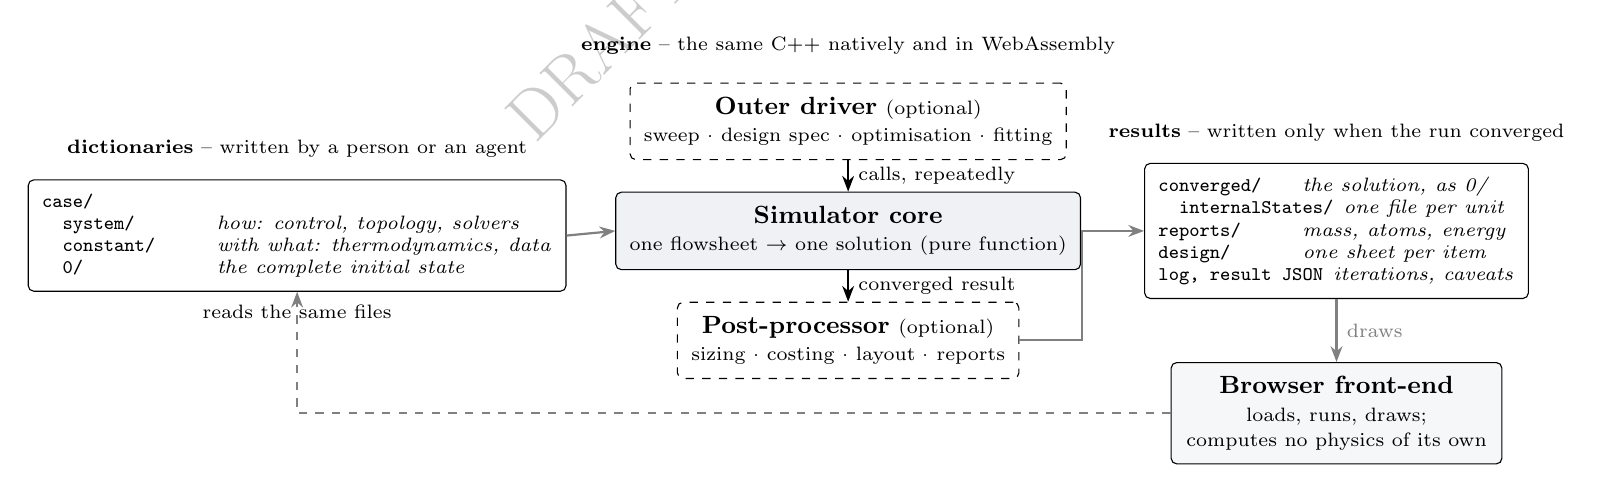
\begin{tikzpicture}[
    box/.style={draw, rounded corners=2pt, align=center, font=\small,
                inner sep=5pt},
    lay/.style={box, minimum width=4.2cm, minimum height=0.85cm},
    opt/.style={lay, dashed},
    arr/.style={-{Stealth[length=2mm]}, thick},
    node distance=0.4cm]
  % the dictionaries
  \node[draw, rounded corners=2pt, align=left, font=\scriptsize\ttfamily,
        inner sep=5pt] (case) {%
    case/\\
    \ \ system/\ \ \ \ \ \ \ \ \textrm{\itshape how: control, topology, solvers}\\
    \ \ constant/\ \ \ \ \ \ \textrm{\itshape with what: thermodynamics, data}\\
    \ \ 0/\ \ \ \ \ \ \ \ \ \ \ \ \ \textrm{\itshape the complete initial state}};
  \node[font=\scriptsize, align=center, above=0.15cm of case]
    {\textbf{dictionaries} -- written by a person or an agent};
  % the engine
  \node[opt, right=0.8cm of case, yshift=1.45cm] (outer)
    {\textbf{Outer driver} \scriptsize(optional)\\[-1pt]
     \scriptsize sweep · design spec · optimisation · fitting};
  \node[lay, below=of outer, fill=linkink!7] (core)
    {\textbf{Simulator core}\\[-1pt]
     \scriptsize one flowsheet $\rightarrow$ one solution (pure function)};
  \node[opt, below=of core] (post)
    {\textbf{Post-processor} \scriptsize(optional)\\[-1pt]
     \scriptsize sizing · costing · layout · reports};
  \draw[arr] (outer) -- node[right, font=\scriptsize]{calls, repeatedly} (core);
  \draw[arr] (core) -- node[right, font=\scriptsize]{converged result} (post);
  \node[draw=none, fit=(outer)(core)(post), inner sep=6pt] (engine) {};
  \node[font=\scriptsize, align=center, above=0.02cm of engine]
    {\textbf{engine} -- the same C++ natively and in WebAssembly};
  \draw[arr, gray] (case.east) -- (core.west);
  % the results
  \node[draw, rounded corners=2pt, align=left, font=\scriptsize\ttfamily,
        inner sep=5pt, right=0.8cm of core] (res) {%
    converged/\ \ \ \ \textrm{\itshape the solution, as 0/}\\
    \ \ internalStates/\ \textrm{\itshape one file per unit}\\
    reports/\ \ \ \ \ \ \textrm{\itshape mass, atoms, energy}\\
    design/\ \ \ \ \ \ \ \textrm{\itshape one sheet per item}\\
    log, result JSON\ \textrm{\itshape iterations, caveats}};
  \node[font=\scriptsize, align=center, above=0.15cm of res]
    {\textbf{results} -- written only when the run converged};
  \draw[arr, gray] (post.east) -| ($(post.east)!0.5!(res.west)$) |- (res.west);
  % the GUI
  \node[box, below=0.8cm of res, minimum width=4.2cm, fill=linkink!4] (gui)
    {\textbf{Browser front-end}\\[-1pt]
     \scriptsize loads, runs, draws;\\[-2pt]
     \scriptsize computes no physics of its own};
  \draw[arr, gray] (res.south) -- node[right, font=\scriptsize]{draws} (gui.north);
  \draw[arr, gray, dashed] (gui.west) -| ($(case.south)+(0,-0.3)$) -- (case.south);
  \node[font=\scriptsize, below=0.05cm of case, xshift=0.0cm, align=center]
    {reads the same files};
\end{tikzpicture}}
\caption{Dictionaries, engine, results and front-end.  The three layers of
the engine; dashed layers are optional.  The front-end runs the same
compiled engine in the browser and draws what it published.}
\label{fig:arch}
\end{figure}

The engine has three layers (Figure~\ref{fig:arch}).  The \emph{simulator
core} turns one flowsheet into one solution -- streams, unit results and key
performance indicators -- as a pure function of its inputs.  An optional
\emph{outer driver} calls that function repeatedly: parameter sweeps,
design specifications, optimisation, parameter estimation.  An optional
\emph{post-processor} chain augments a converged solution with equipment
sizing, costing, plant layout and reports.  Five binaries partition the
problem classes (Table~\ref{tab:scope}); numerical strategies coexist inside
each binary and are selected in the case files, so there is no binary per
algorithm.  The whole engine builds with \code{g++} and GNU make alone --
369 translation units, no external library -- so that a student can read
every line that computes: the Newton solvers (one- and $n$-dimensional),
Wegstein on declared tear streams, Nelder--Mead, Michelsen's stability test,
RK4 and a Rosenbrock23 integrator for stiff dynamics are all in
\code{src/solver/}, every iteration printed at the default verbosity, and
convergence is decided by one normalised residual with an \OF-shaped
(\code{tolerance}, \code{relTol}, \code{maxIter}) triple declared per
solver.  The time-integrated classes share one driver: \code{choupoBatch}
adds a recipe of timed events and two campaign ledgers (material and
energy, every integral an exact state difference), \code{choupoSemiContinuous}
a quasi-steady adapter that re-solves any steady unit inside a transient,
and \code{choupoCtrl} PID, schedule and signal controllers with a balance
ledger on the integrator's accepted steps.
% make/compiler.mk:35-40 (CXX g++, -std=c++17); `find src -name '*.cpp' |
% wc -l` = 369 at feb112a00; CLAUDE.md sec 2 ("Zero external dependencies")
% and sec 10 "No external libs"; src/solver/ (NewtonRaphson, NewtonND,
% Wegstein, NelderMead, StabilityTest, ODE/RK4, ODE/Rosenbrock23);
% src/solver/Convergence.H (the triple, the normalisation); CLAUDE.md sec 6
% "Batch campaign LEDGERS" (TransferRecord, EnergyRecord, exact state
% differences), sec 10 "THE QUASI-STEADY SEAM (#185)" (src/dynamicDriver/
% DynamicDriver.cpp:350-384 `quasiSteady`), src/control/ (PIDController,
% ScheduleController, SignalController), DynamicDriver.cpp:885-925 (the
% accepted-step trapezoid ledger), gate check_ctrl_balance.
% CLAUDE.md sec 4 ("Architecture: 3 layers"); the pure function is
% runSimulation, src/applications/choupoSolve/main.cpp:145, called by the
% direct path (:1222) and by every outer driver's functor (:894); CLAUDE.md
% sec 10 "One binary per problem class"; src/dynamicDriver/ is the one home
% the two dynamic binaries share (CLAUDE.md sec 4 source tree).

\paragraph{Explicit factories.}  Every extensible base class -- unit
operations, activity models, equations of state, vapour-pressure and
heat-capacity models, transport correlations, outer drivers,
post-processors, sizers, property operations -- has a factory, and every
built-in type is registered by one line inside a \code{registerBuiltins()}
function that \code{main()} calls explicitly.  There are no
self-registration macros and no static initialisers, so ``where does this
model come from?'' is answered by reading one function.  The cost is
stated: a new built-in needs one registration line and a rebuild.
% CLAUDE.md sec 5 "Factory pattern -- always explicit"; the calls in
% src/applications/choupoSolve/main.cpp:443-465; the flash's registration
% line src/unitOperations/UnitOperation.cpp:157; the factory signature
% src/unitOperations/UnitOperation.H:228-237.

\paragraph{A user can write their own unit operations and models.}  On a
local installation, a case may ship its own \code{code/} directory: a
class and one registration line in \code{registerUserTypes()}, the hook
\code{main()} calls right after the built-ins are registered, compiled
against the engine by \code{bin/buildCode} with a plain, printed
\code{g++} command and linked into a per-case binary.  It is the same
mechanism the project uses to add a built-in -- the same factory, the same
explicit line -- so a student's unit operation is not a second-class
plug-in.  Two tutorials do exactly this: \code{userOp01_yield_reactor}
registers a unit operation, \code{userOp03_case_rate_law} a rate law,
which it also writes a second way, as an \emph{expression} in the case's
own \code{constant/reactions} over declared parameters with units,
compiled by the engine's formula evaluator with no C++ at all; and any unit
may carry a \code{thermo {}} block that replaces the global
thermodynamic models for that unit alone.  The hosted site runs the shipped
engine only -- there is no compiler in the browser -- so the \code{code/}
route is the local installation's privilege; the expression route and the
per-unit override work in both.
% src/applications/choupoSolve/main.cpp:134-138 (the stub) and :465
% (registerUserTypes() called after the builtins); bin/buildCode:88, :173-178
% ("plain build-time g++, nothing hidden, no runtime dlopen");
% tutorials/steady/userops/userOp01_yield_reactor/code/registerUserTypes.cpp:19
% (UnitOperation::registerType) and userOp03_case_rate_law/code/
% registerUserTypes.cpp:20 (ReactionRate::registerType; its header: "the
% same explicit factory the built-ins use --- no macro self-registration");
% userOp03's constant/reactions:47 (`type expression;`); CLAUDE.md sec 5
% "Adding a new unit operation" (CLAUDE.md:517) and "Per-unit `thermo {}`
% override"; CLAUDE.md sec 6 "A CASE CARRIES ITS OWN KINETICS" (C67: "or a
% law a case's `code/` registers (local only: the site has no compiler)",
% CLAUDE.md:2107).

\paragraph{State directories are restartable snapshots.}  The steady
solution is written to \code{converged/} in the same layout as \code{0/},
and only when the run converged: the directory's name is a contract.  Each
unit's internal state (a column's stage profile, a reactor's axial profile,
a crystal size distribution) is written beside the streams under
\code{internalStates/}, one file per unit, so a converged directory renamed
\code{0/} restarts the case from its answer.  The time-integrated binaries
write a time directory at every write interval in the same layout.
\code{iterations/} keeps the numerical history when asked for, and is never
physical time.  A case can also be \emph{sealed}: \code{bin/choupo-import}
copies the full closure of property records the case consumes into its own
\code{constant/} under a manifest with a checksum per record, and a sealed
case runs with the installation catalogue forbidden to it, so a tutorial
answers the same on any machine; the seal is computational -- it compares
parsed content, not bytes, so a comment moved is cosmetic and a value moved
is a refusal -- and every tutorial in the corpus is sealed.
% CLAUDE.md sec 6 "General heterogeneous-thermo solver" (SEALED
% constant/propertyManifest, per-record sha256, "the runtime is FORBIDDEN
% the installation catalogue when sealed") and "The seal is COMPUTATIONAL
% since 2026-08-03" (sealSchema computational; gate check_seal_schema);
% src/thermo/SealCheck.cpp:127; src/thermo/RecordResolver.H:337; the
% flash01 case carries constant/propertyManifest (ls, feb112a00).
% src/applications/choupoSolve/main.cpp:1077-1078 (writeConverged returns
% unless result.converged); CLAUDE.md sec 3 (state views hold both halves;
% time-integrated classes write <t>/ by default; record docs/design/
% a-state-directory-is-a-restartable-snapshot.md sec 9-11);
% src/io/SolutionWriter.cpp:521 (iterations/); src/dynamicDriver/
% DynamicDriver.cpp:499 (writeInterval).

\paragraph{A plant and its sectors.}  A large flowsheet may be organised as
a plant and its sectors, each sector a folder with its own \code{system/}
and \code{constant/}; the engine flattens the tree to one flat problem with
qualified names, and a sector may declare its own thermodynamic model.  The
reference case runs five sectors across four thermodynamic models (an
electrolyte Pitzer brine, an NRTL liquid--liquid split, a Gibbs reactor and
a molecular section) and closes its atom balance on every element; a
stream crossing from one model to the next is re-priced there, and the
enthalpy step is \emph{accounted} in a model-boundary ledger of its own
rather than charged to the unit that received it.
% CLAUDE.md sec 6 "THE MODEL-BOUNDARY STEP IS ACCOUNTED, NOT CHARGED TO THE
% UNIT" (raw imbalance, declared step, what remains); src/reporting/
% ModelBoundaryLedger.H:141 (modelBoundaryClosure); gate
% check_model_boundary_ledger; record docs/design/
% model-boundary-energy-ledger.md.
% src/unitOperations/flowsheet/Flowsheet.cpp:256 (flattenNode); CLAUDE.md
% sec 3 (a plant and its sectors); sec 6 "General heterogeneous-thermo
% solver" (tutorials/plant/lithiumBrinePlant: 5 sectors, 4 worlds, mass
% closes on every element).

\subsection{The browser front-end is a visualiser, on the ParaView pattern}
\label{sec:gui}

In the usual process-simulator workflow the user \emph{builds} the case in
the graphical interface.  Choupo does the opposite, on the pattern of
\OF\ and ParaView: \OF\ computes, and ParaView shows what was computed.
Choupo computes -- natively, or in WebAssembly from the same C++ -- and the
browser front-end shows the case so that the user understands it.  The
case is always text dictionaries, authored in an editor or with an agent;
the front-end loads them, draws them, runs the engine on them and shows
what the engine published, and nothing it shows is computed by the
front-end itself.  That stance was settled before the first screen was
drawn and is the front-end's design rule: it is a viewer, not a block
editor and not an IDE.  Pressing F1 on any view opens the guide at the
section that derives it.
% CLAUDE.md sec 12 (CLAUDE.md:4088-4094: "Design stance (settled
% 2026-05-16, codified as a Credo): the GUI is a runner and visualiser, NOT
% an editor -- cases are authored as plain-text dicts on disk ... ParaView-
% inspired but with its OWN identity"); docs/ai/gui-credo.md:7-28 (informed
% by "ParaView's separation of authoring (offline) from viewing (in the
% GUI)"; "The Choupo GUI is a viewer for a Choupo case directory"; not a
% block editor, not a literal ParaView clone, not an IDE; "The GUI shows
% what is on disk; it does not write back silently"); make/wasm.mk:25-39
% (all five binaries to gui/public/wasm/); gui/src/ui/AppShell.tsx:234-245
% (F1).  ParaView is Kitware's open-source visualiser; its name is not on
% check_doctrine's ban list (bin/curate/check_doctrine.py:67-68).

What it shows, in the version cited here: the flowsheet, with each stream
coloured by the phase the engine resolved for it; the run log, streamed
live while the engine runs; the three global balances -- mass, atoms,
energy -- drawn from the engine's own reports and never recomputed (the
rule since the day the front-end's own first-law sum was found to disagree
with the engine's by an order of magnitude); a plant and its sectors, each
sector openable as a case of its own; the stream table and each unit's
results and profiles; the specification sheets under \code{design/} -- one
dictionary per sized item, regenerated every run, each value with its unit
and its design basis and an \code{assumed} line naming what the case did
not declare -- drawn as a datasheet by equipment kind; the Explorer -- the
compound catalogue, an inspector with provenance marks, an estimate form,
and property surfaces ($T$-$x$-$y$, $\gamma$, $P^\mathrm{sat}$, LLE, ternary,
Gibbs maps, Bjerrum, steam tables, transport, phase envelopes, Hildebrand
parameters), with an Evidence view that draws measured points against
candidate models being merged; the EduTools; and the plant layout in 3D --
the plot plan with the case's declared separations and zones, pipes routed
orthogonally on a rack, the plot area, roads and site buildings, a fence
with gates, a truck route walked against a declared vehicle, the GMP
building interior -- all declared by the case, checked by the engine and
drawn by the front-end, each item by its equipment kind on the envelope
the engine published and, today, sitting at grade (foundations and the
final piping detail are future work).  The next step on the development line, in
the sense of Section~\ref{sec:limits}'s evolution paragraph and not of the
cited version, is the instrumented flowsheet: a P\&ID layer declared over
the PFD -- loops, transmitters, control valves, ISA tags -- validated by
the engine, drawn by the front-end as a second view, and used as the input
from which \code{choupoCtrl} runs the same case with its control loops.
% gui/src/ui/FlowCanvas.tsx:138-145 (stream colour from the engine's vapour
% fraction, "vf is the AUTHORITATIVE phase signal"); LogWorkspace.tsx:171
% (follow live output while solving); ReportsWorkspace.tsx and
% StreamsSummary.tsx (globalEnergyBoundary read, not computed) and
% docs/design/a-first-law-the-gui-computed-for-itself.md (372.5 kW vs the
% engine's 34.4 kW, 2026-09-05); CaseWorkspace.tsx:333-344 (a sector opened
% as a case of its own); StreamsTable.tsx, UnitStreamsTable.tsx,
% PlotsWorkspace.tsx; ReportsWorkspace.tsx:37-54 (design/ "exactly as the
% engine wrote them"); ExploreWorkspace.tsx, CompoundCatalogue.tsx;
% MethodsWorkspace.tsx (EduTools); LayoutPopOutTab.tsx:69 (PlantLayout3D,
% three.js) and CLAUDE.md sec 6 "A PLANT LAYOUT IS DECLARED, CHECKED AND
% DRAFTED" (C75, C88: each item by its equipment kind on the published
% envelope).  The P&ID: DEV.md 4c C130 on origin/main (f8d09d205, Vitor:
% the P&ID "deve ser usado para correr o choupoCtrl"; proposed and
% measured, NOT in the cited version).

\subsection{What Choupo takes from \OF, and where it differs}
\label{sec:openfoam}

Choupo's case organisation is inspired by
\OF\textsuperscript{\textregistered}\footnote{OPENFOAM\textsuperscript{\textregistered}
is a registered trade mark of OpenCFD Limited, producer and distributor of
the OpenFOAM software via www.openfoam.com.}
\citep{weller1998}, the open-source C++ toolbox for continuum mechanics
whose plain-text dictionaries and case directories we regard as one of the
most elegant designs in scientific software.  Table~\ref{tab:openfoam} maps
the concepts one to one and says, for each, whether Choupo does the same
thing or something different and why.  \textbf{Choupo is an independent
project: it is not part of, affiliated with, endorsed by or sponsored by
OpenCFD Ltd or the OpenFOAM Foundation, and no \OF\ source code was adapted
or reused in it.}  \emph{This offering is not approved or endorsed by
OpenCFD Limited, producer and distributor of the OpenFOAM software via
www.openfoam.com, and owner of the OPENFOAM\textsuperscript{\textregistered}
and OpenCFD\textsuperscript{\textregistered} trade marks.}
% The three statements are those OpenCFD's Trade Mark Policy asks of third
% parties (https://www.openfoam.com/opencfd-limited-trade-mark-policy, read
% 2026-10-21: the registration mark on the first reference, point 4; the
% Acknowledgement, point 4; the Disclaimer, point 3; the marks used in their
% registered form, point 11).  Independence: NOTICE:127-140 (provenance
% review of the dictionary parser, the factories, the Rosenbrock23
% integrator and the time-directory writer: independent implementations);
% docs/developerGuide.tex:55-64.

\begin{table}[htbp]
\centering\scriptsize
\caption{\OF\ concepts and their Choupo equivalents.}
\label{tab:openfoam}
\renewcommand{\arraystretch}{1.1}
\begin{tabularx}{\linewidth}{>{\raggedright\arraybackslash}p{3.3cm}
                             >{\raggedright\arraybackslash}p{3.6cm}
                             >{\raggedright\arraybackslash}X}
\toprule
\textbf{\OF\ concept} & \textbf{Choupo equivalent} & \textbf{Same, or differs because} \\
\midrule
A case is a directory: \code{system/}, \code{constant/}, \code{0/} &
  the same three directories & Same.  \code{system/} holds control, topology
  and solver dictionaries; \code{constant/} the thermophysical system;
  \code{0/} the complete initial state. \\
Hierarchical plain-text dictionaries, \code{keyword value;};
  \code{controlDict} with \code{writeInterval} &
  the same grammar and the same control file & Same.  Choupo requires a
  unit or a dimension set on every dimensional scalar and converts to SI on
  reading; \code{writeInterval} drives the time-integrated binaries, and
  the steady one writes \code{converged/} once, only on convergence. \\
A field file carries \code{internalField} and \code{boundaryField} &
  a state view carries the streams (the boundary) and
  \code{internalStates/<unit>} (the interior) & Same idea, one level up: a
  stream is an edge between units, a unit's profile is its interior, and
  both are needed to restart. \\
Time directories \code{0.1/}, \code{0.2/} &
  \code{<t>/} in the dynamic binaries; \code{iterations/} for numerical
  history & Same for physical time.  Differs: a steady run keeps its
  iteration history under a separate name, so a directory named by a number
  always means time. \\
One application per solver algorithm (\code{icoFoam},
  \code{simpleFoam}, \ldots) &
  one application per \emph{problem class} (five binaries) & Differs: a
  flowsheet's numerical strategy (Newton, Wegstein, Nelder--Mead, \ldots) is
  chosen in the case, so a student changes the method without changing
  the program. \\
Run-time selection through registration macros and static tables &
  explicit \code{registerBuiltins()} functions called from \code{main()} &
  Differs by design: no macro and no static initialiser, so the origin of
  every model is one readable function; the cost is one line and a rebuild
  per built-in. \\
Residual normalisation (\code{normFactor}) &
  \code{solver/Convergence.H}: the same structure with equations in place
  of cells & Same structure and intent; the header states the three places
  where the analogy stops (a single-equation system degenerates and falls
  back to the raw residual, announced). \\
\OF\ computes; ParaView shows what was computed &
  the engine computes; the browser front-end shows the case and the result &
  Same pattern (Section~\ref{sec:gui}): the case is text, the viewer
  computes nothing. \\
Compiled utilities (\code{blockMesh}, \code{foamDictionary}, \ldots) &
  small scripts and tools in \code{bin/} (\code{runCase},
  \code{choupo-init0}, \code{choupo-lint}, \ldots) & Differs: Choupo's
  utilities are mostly scripts around the five binaries. \\
Default branch is the development line; releases are versioned tags
  (\code{OpenFOAM-dev}, \code{OpenFOAM-13}) &
  \code{main} is \code{Choupo-dev}; a release is an immutable tag
  \code{vYYMM} & Same, adopted after checking that project's repositories
  rather than from memory. \\
\bottomrule
\end{tabularx}
\end{table}
% Rows: CLAUDE.md sec 3 (layout), sec 5 (dictionaries, units), sec 3
% "THE TIME-INTEGRATED CLASSES ... WRITE <t>/ BY DEFAULT" and "A STATE VIEW
% HOLDS BOTH HALVES" (internalField/boundaryField analogy, CLAUDE.md:268),
% src/io/SolutionWriter.cpp:521 (iterations/), CLAUDE.md sec 10 "One binary
% per problem class", sec 5 "Factory pattern -- always explicit",
% src/solver/Convergence.H:84-105 (normFactor with cells -> equations; "NOT
% the same theorem.  Three honest limits"), CLAUDE.md sec 2 "Branches & tags"
% (OpenFOAM.org checked at 09951d6: default branch = the line's own;
% sec 10 C++17 paragraph: "checked ... on every platform rule in the tree").
% The OpenFOAM-side facts (one application per solver, registration macros,
% compiled utilities, dimensionSet, normFactor, OpenFOAM-dev) are that
% project's public documentation and source; the OpenFOAM contributor in the
% reader forum confirmed the first three.

\FloatBarrier
%===============================================================================
\section{Thermophysical data}
\label{sec:data}

\subsection{A source and a licence for every value}

The curated catalogue (\code{data/standards/}) cites the primary source per
value, never an aggregator's arrangement; each record says where its
numbers came from and how they were obtained (measured, regressed,
estimated), and a record that has not been reviewed, or that comes from the
user's private local tier, is announced as such every time a run reads it.
Licence classes are decided before a value enters the tree: a dataset with
no licence statement is treated as no-grant and kept out; a NonCommercial
grant is kept out, because Choupo is free for commercial use; a pair table
does not acquire its courier's licence by being redistributed inside a
permissively licensed package.  The engine refuses to write into the
curated catalogue: new data enters it by a human act of curation, and a
gate (defined in Section~\ref{sec:vv}) holds every record to these rules.
% CLAUDE.md sec 10 licence policy (CODE vs DOCS vs DATA; NonCommercial and
% no-grant excluded; cite the PRIMARY source per value); sec 7 (two data
% tiers; [local] UNVERIFIED); src/thermo/Database.cpp:605 ("[unreviewed]
% component"); docs/design/the-licence-of-a-sigma-profile.md (silence is not
% permission); docs/design/binary-pairs-from-open-measurements.md sec 1 (a
% pair table is not freed by its courier's licence);
% records::refuseStandardsWrite, src/thermo/RecordResolver.H:236, gate
% check_standards_write_guard; gate check_source_licence (claim at
% 31f6a56ab: "1180 record(s) scanned ... no encumbered source stands as the
% authority for a value, except 4 pinned violations awaiting curation").

\subsection{The curation tools, and what a promoted record carries}

Curation is a chain of commands, each leaving a file a reader can open.
\code{bin/choupo-thermoml} locates measured data in the open NIST/TRC
ThermoML archive -- joined to the catalogue by InChIKey, never by name --
and extracts a dataset that names its article, its DOI, the archive file
and block, the per-point uncertainty and a review status.  \code{choupoProps}'
\code{fitParameters} operation regresses a model's parameters on datasets
declared as \emph{fit} and scores them on datasets declared as
\emph{held-out}, against an acceptance band declared \emph{before} the fit;
\code{evidencePartition} announces how independent the two roles are;
\code{vleConsistency} tests a dataset's thermodynamic consistency; the
\code{curationDossier} records what was used, excluded and assumed.  The
fit writes a \emph{proposal} record and promotes nothing: promotion into
the catalogue is a human act (\code{bin/curate/promote-from-dossier}),
and a promoted record carries its evidence, its validity span and its
verdict, so a gate can re-run its case and refuse a record that drifts from
what produced it.
% CLAUDE.md sec 6 "ONE THERMOML TOOLCHAIN" (identity, vle-index, vle-search,
% extract-vle; InChIKey join) and "A PAIR CHOUPO REGRESSES IS A RECORD THAT
% NAMES ITS CASE"; src/propertyOps/PropertyOperation.cpp:188 (fitParameters)
% and :201 (vleConsistency); src/propertyOps/EvidencePartition.cpp:465-472
% (the identity-level independence facts, ANNOUNCED); bin/choupo-curate,
% bin/curate/promote-from-dossier (exist at feb112a00); DEV.md 4c C117 (the
% pipeline as it exists); gate check_regressed_pairs (re-runs each record's
% case and holds the record to it).
Listing~\ref{lst:record} is the validation block of one promoted pair, with
the sentence that says where its acceptance band came from.

\Needspace{20\baselineskip}
\begin{lstlisting}[caption={The \texttt{validation} block of the promoted
  NRTL record for 1-propanol + water
  (\texttt{data/standards/parameters/NRTL/1Propanol-water.dat}; the
  \texttt{origin} sentence shortened at \texttt{[...]}).},label=lst:record,
  breaklines=true]
validation
{
    verdict     validated;
    heldOut
    {
        points      19;
        aad_pct     0.056538;
        aad_K       0.205310;
        domain_x1   ( 0.058000 0.976000 );
    }
    acceptance
    {
        maxAAD      0.260000;   // per cent
        origin      "declared before the fit, by the ONE rule of C16 [...]: the held-out set's largest stated expanded uncertainty (U95 = 0.22 K) plus the catalogue vapour-pressure model's own error at that set's pure endpoints (water -0.703 K, 1Propanol +0.051 K; measured with no pair involved), as a percentage of the held-out mean T (362.46 K) = 0.2546 %, rounded UP to two significant figures";
    }
}
\end{lstlisting}
% data/standards/parameters/NRTL/1Propanol-water.dat at feb112a00, the
% `validation {}` block verbatim except the elision marked.  The same
% record's provenance block names the two articles (DOIs 10.1021/je800436u
% for the fit, 10.1016/j.jct.2017.06.014 held out), each dataset's sha256,
% the fitting case (curate09) and the validity span (360.49-368.64 K).

\subsection{A worked example: who does what, and a candidate that fails}
\label{sec:worked}

The example is the acetone + methanol pair, chosen because it is the
azeotrope a student meets in two plants of the tutorial corpus and because
it is the one of nine regressed pairs that \emph{failed} its test.  The
division of responsibilities is the point.
% tutorials/props/curation/curate05_nrtl_acetone_methanol/system/propsDict
% header ("WHY THIS SYSTEM"; "WHAT THE RUN FOUND"); DEV.md 4c C16 (slice 1:
% four validated and promoted, acetone-methanol NOT validated; slice 2: four
% more validated, three promoted).

\begin{description}[leftmargin=1.6em, itemsep=3pt]
\item[The user] states the problem: the mixture (acetone, methanol), the
  property (bubble temperature of the binary at atmospheric pressure, the
  quantity a distillation column needs), and the conditions (near
  101~kPa, the whole composition range).
\item[The agent] finds the evidence and organises it.  \code{choupo-thermoml}
  locates two independent isobaric studies in the archive, one at
  101.3~kPa \citep{chen2015} and one at 100~kPa \citep{orchilles2007},
  extracts each with its per-point uncertainty (0.1--0.35~K), sets the pure
  endpoints aside (they test the vapour-pressure record, not the pair) and
  writes a \code{propsDict} that declares the larger study as the fit set
  and the other as held out, two NRTL parameters ($b_{ij}$, $b_{ji}$;
  $\alpha$ fixed at 0.30), uncertainty weighting, and the acceptance band.
  The band is computed by one rule applied to every pair before any fit
  runs: the held-out set's largest stated uncertainty plus the catalogue
  vapour-pressure model's own error at the pure ends, as a percentage of
  the held-out mean temperature -- here 0.047~\%, 0.155~K.  The agent then
  runs the fit.
\item[The engine] records what was used and excluded (the two datasets with
  DOI, archive file, checksum and review status, the endpoints set aside),
  freezes a fingerprint of the partition before the regression starts,
  announces that neither dataset has been read back against its article,
  fits by Levenberg--Marquardt (and again from a second start, landing on
  the same pair), reports the in-sample residual, and computes the held-out
  verdict against the declared band.  It also runs three bubble-point
  scans -- ideal, UNIFAC, the fitted NRTL -- at each study's pressure and
  overlays both studies on them.
\item[The interface] shows the measurements, the model curves, the
  residuals per point and the limits of use: Figure~\ref{fig:fit}, drawn
  from the run's own files.
\item[The student] reads the dictionaries and the dossier, compares the
  alternatives on the figure and justifies a choice.
\end{description}

\begin{figure}[t]
\centering
% Data: paper/whitepaper/data/*.csv, the curate05 run's own outputs (see the
% RUNS comment at the top of this file).  Left: the FIT study at 101.3 kPa
% (exp_fitset_acetone_methanol.csv) with the engine's scans at that pressure
% (txy_nrtl_fitP.csv, txy_unifac_fitP.csv, txy_ideal_fitP.csv) and the fit
% residuals the engine wrote (parity.csv, column `residual` = T_model -
% T_exp).  Right: the HELD-OUT study at 100 kPa
% (exp_heldout_acetone_methanol.csv) with the scans at 100 kPa (txy_*.csv)
% and the residuals of heldout_residuals.csv (interpolated from the scans at
% the measured x).  The band is the declared 0.047 % of 330.21 K = 0.155 K.
\pgfplotsset{every axis/.append style={font=\scriptsize, tick label style={font=\scriptsize}}}
\begin{tikzpicture}
\begin{groupplot}[group style={group size=2 by 2, horizontal sep=1.3cm,
                   vertical sep=0.55cm, x descriptions at=edge bottom},
                  width=7.4cm]
  % --- top left: fit study, 101.3 kPa
  \nextgroupplot[height=4.6cm, ylabel={$T_\mathrm{bubble}$ [K]},
                 title={\textbf{Fit study}, 101.3 kPa, 32 points},
                 ymin=327, ymax=338.5, xmin=0, xmax=1,
                 legend style={at={(0.97,0.97)}, anchor=north east, font=\tiny,
                               draw=none, fill=none}, legend cell align=left]
    \addplot[idealink, densely dotted, thick] table[col sep=comma, x index=0, y index=1]
      {data/txy_ideal_fitP.csv};
    \addlegendentry{ideal}
    \addplot[unifacink, dashed, thick] table[col sep=comma, x index=0, y index=1]
      {data/txy_unifac_fitP.csv};
    \addlegendentry{UNIFAC (predictive)}
    \addplot[fitink, thick] table[col sep=comma, x index=0, y index=1]
      {data/txy_nrtl_fitP.csv};
    \addlegendentry{NRTL, fitted here}
    \addplot[only marks, mark=square*, mark size=1.6pt, fitink]
      table[col sep=comma, x index=0, y index=1] {data/exp_fitset_acetone_methanol.csv};
    \addlegendentry{measured, FIT set}
  % --- top right: held-out study, 100 kPa
  \nextgroupplot[height=4.6cm,
                 title={\textbf{Held-out study}, 100 kPa, 30 points},
                 ymin=327, ymax=338.5, xmin=0, xmax=1,
                 legend style={at={(0.97,0.97)}, anchor=north east, font=\tiny,
                               draw=none, fill=none}, legend cell align=left]
    \addplot[idealink, densely dotted, thick] table[col sep=comma, x index=0, y index=1]
      {data/txy_ideal.csv};
    \addlegendentry{ideal}
    \addplot[unifacink, dashed, thick] table[col sep=comma, x index=0, y index=1]
      {data/txy_unifac.csv};
    \addlegendentry{UNIFAC (predictive)}
    \addplot[fitink, thick] table[col sep=comma, x index=0, y index=1]
      {data/txy_nrtl.csv};
    \addlegendentry{NRTL, fitted on the left}
    \addplot[only marks, mark=o, mark size=1.7pt, heldink, thick]
      table[col sep=comma, x index=0, y index=1] {data/exp_heldout_acetone_methanol.csv};
    \addlegendentry{measured, HELD-OUT set}
  % --- bottom left: fit residuals (NRTL)
  \nextgroupplot[height=3.6cm, xlabel={$x_\mathrm{acetone}$},
                 ylabel={$T_\mathrm{model}-T_\mathrm{exp}$ [K]},
                 ymin=-0.6, ymax=0.6, xmin=0, xmax=1, ytick={-0.4,0,0.4}]
    \addplot[gray!60, fill=gray!15, draw=none] coordinates {(0,-0.155) (1,-0.155) (1,0.155) (0,0.155)} \closedcycle;
    \addplot[black!60, thin] coordinates {(0,0) (1,0)};
    \addplot[only marks, mark=square*, mark size=1.5pt, fitink]
      table[col sep=comma, x index=0, y index=4] {data/parity.csv};
    \node[font=\tiny, anchor=south west] at (axis cs:0.02,0.36)
      {NRTL on its own fit set: AAD 0.10 K};
  % --- bottom right: held-out residuals (NRTL and UNIFAC)
  \nextgroupplot[height=3.6cm, xlabel={$x_\mathrm{acetone}$},
                 ymin=-0.6, ymax=0.6, xmin=0, xmax=1, ytick={-0.4,0,0.4},
                 legend style={at={(0.03,0.95)}, anchor=north west, font=\tiny,
                               draw=none, fill=none}, legend cell align=left,
                 legend columns=2]
    \addplot[gray!60, fill=gray!15, draw=none] coordinates {(0,-0.155) (1,-0.155) (1,0.155) (0,0.155)} \closedcycle;
    \addplot[black!60, thin] coordinates {(0,0) (1,0)};
    \addplot[only marks, mark=o, mark size=1.6pt, fitink, thick]
      table[col sep=comma, x index=0, y index=2] {data/heldout_residuals.csv};
    \addlegendentry{NRTL, AAD 0.316 K}
    \addplot[only marks, mark=triangle, mark size=1.7pt, unifacink, thick]
      table[col sep=comma, x index=0, y index=3] {data/heldout_residuals.csv};
    \addlegendentry{UNIFAC, AAD 0.041 K}
\end{groupplot}
\end{tikzpicture}
\caption{The acetone + methanol regression, drawn from the run's own files.
Top: bubble-point curves of three models at each study's pressure, with the
study the NRTL pair was fitted to (left, filled squares) and the study it
was held out on (right, open circles) -- two laboratories, two articles, no
author in common.  Bottom: residuals per point; the grey band is the
acceptance band declared before the fit ($\pm 0.155$~K).  The fitted pair
reproduces its own study to 0.10~K and misses the other by 0.316~K; UNIFAC,
which saw neither, does the mirror image (0.34~K on the fit study, 0.041~K
on the held-out one).  The verdict is \texttt{notValidated}, and the pair
was not promoted.}
\label{fig:fit}
\end{figure}

What the student sees in Figure~\ref{fig:fit} is a candidate that fits its
training data well and fails its test.  The fitted NRTL pair reproduces the
study it was fitted to with an rms of 0.13~K and an average deviation of
0.10~K; on the other study its average deviation is 0.316~K (0.096~\%),
twice the band declared before the fit, so the verdict is
\code{notValidated} and the record stays in the case rather than entering
the catalogue.  UNIFAC, a predictive model that saw neither study,
reproduces the held-out study to 0.041~K and misses the fit study by
0.34~K.  The two studies disagree with each other by about 0.3~K where each
states 0.1--0.35~K; which is right is a question for a curator who reads
both articles, not for the fitting tool.  Swapping the roles of the two
studies after seeing the residuals would be the tuning the declared
partition exists to prevent; the engine's fingerprint of the partition,
frozen before the fit, is what makes that visible.
% Numbers: the curate05 run of 2026-10-21 (log lines "Final chi2
% 4.45237e+00", "rms 0.126864", "AAD 0.0960 % (0.3160 K)", "maxAAD 0.0470 %",
% "notValidated"; the overlay AADs txy_unifac 0.0408 K held-out / 0.3404 K
% fit set, txy_nrtl 0.3160 / 0.1010 K, txy_ideal 2.8641 / 3.3657 K), equal to
% the case's pinned golden (curate05/expected rows diag aad_heldout_K
% 0.315969383935, verdict notValidated, aad rows 70-87) and byte-identical
% to an independent run of the same case by another worker.  The 0.3 K
% disagreement between studies and the curator's remedy: the case's own
% header ("WHY, as far as the run can see").

The student who must choose a model for the column now has grounds: at
these pressures UNIFAC describes the independent measurement better than
the regressed pair; both place the azeotrope at $x_\mathrm{acetone}
\approx 0.78$ at 100~kPa, so a column design is not sensitive to the choice
there; and neither has been tested at the 6~atm of a pressure-swing
scheme, which the engine will announce as an extrapolation of the pair's
evidence if it is run there.  A second candidate in the same corpus fails
the other way: the ethanol + cyclohexane pair \emph{passed} its held-out
band (0.094~\% against 0.41~\%) and was still not promoted, because the
same parameters predict a liquid--liquid split across the whole of their
validity span where both studies report one liquid.  A bubble-temperature
scan solves for one liquid by construction, so its verdict cannot see a
second: \emph{validated} is necessary, not sufficient, and the catalogue
gate holds every promoted pair to one liquid across its span.
% Azeotrope from the 100 kPa scans (txy_nrtl.csv, txy_unifac.csv: T minimum
% and y = x crossing between x = 0.77 and 0.78 for both models; measured
% here from the CSVs).  The 6 atm extrapolation: benchmark case B README
% (branch claude/c123-benchmarks-bc 33e277ca2: "about 50-56 K above the
% pair's evidence ... Every run announces the extrapolations ([pair-span],
% [psat], [cp])"); CLAUDE.md sec 6 (C35 item 5: [pair-span] announced).
% Ethanol + cyclohexane: tutorials/props/curation/
% curate12_nrtl_ethanol_cyclohexane/system/propsDict header, its run of
% 2026-10-21 (AAD 0.0940 % (0.3234 K), maxAAD 0.41 %, validated), DEV.md 4c
% C16 slice 2, check_regressed_pairs arm (f).

\FloatBarrier
%===============================================================================
\section{Verification and validation}
\label{sec:vv}

A \emph{gate}, in this project, is an automated check that runs with the
test suite and fails if a specific class of error reappears; each one
prints the single line that states what it checked and what it did not.
% docs/design/which-line-is-a-gates-claim.md; bin/curate/gate_claim.py;
% generated/gateManifest.json (note: "DERIVED by running each gate and
% capturing the line it MARKS as its claim").
The test suite has several kinds of check, and the useful thing to know is
what each kind lets one conclude.

\paragraph{A golden-master pass means ``not moved'', never ``right''.}
Of the 480 runnable cases, 463 carry a reference answer that an earlier
Choupo run recorded, and every suite run compares each case with its
reference (and screens every case for NaN and infinity, because an
exit-code check passes on a silent NaN).  A pass proves the answer has not
moved; it says nothing about whether it was ever right.  A re-recorded
reference is therefore treated as a claim: the rows that moved are listed,
each with the physical or numerical reason, before anything is re-recorded,
and a row that moves for a reason nobody can state is a regression until
proven otherwise.
% generated/releaseInventory.json (c402561ad): runnableCases 480,
% regressionChecks 463; CLAUDE.md sec 10 "When implementing" (NaN/inf guard
% on every case; the bare exit-code check is banned) and "A GOLDEN RE-RECORD
% IS A CLAIM, AND THE CLAIM IS THE LIST"; docs/architecture/
% verification-and-validation.md sec 1.

\paragraph{Validation is a small, named subset.}  Following the distinction
in NASA-STD-7009 \citep{nasa7009}, the project keeps a named list of cases
anchored to independent published results, recounted by a gate on every
run so a case cannot join or leave it unnoticed.  The system-level anchors
are the Williams--Otto reactor and its published steady state
\citep{williams1960}, the IAPWS-IF97 verification tables \citep{wagner2000},
and the Cavett recycle train on its primary specification (the
specification, not a published product table -- the case says so).  The
property-level anchors are mostly aqueous electrolytes: the Hamer--Wu
activity coefficients of uni-univalent salts \citep{hamer1972}, a measured
calcite pH \citep{plummer1982}, Carey--Lewis ethanol--water VLE, and
others; where an anchor is the model's own training data, the row says
``fit-consistency'' and is not counted as validation.  The subset holds no
rigorous column, no recycle plant and no liquid--liquid flowsheet anchored
to a measurement, and today only five cases carry \emph{anchor} rows the
suite falsifies by machine; the rest of the table is a claim in prose.
Section~\ref{sec:ex-research} adds the membrane anchors, which are held by
their own gates.
% docs/architecture/verification-and-validation.md sec 3 (tables A and B
% with each row's independence; "exactly five cases use [anchor rows]";
% "Every other row here is still a claim in prose"); gate
% check_validation_subset (claim at 31f6a56ab: membership recounted; "NOT
% CHECKED: whether any anchor is RIGHT").

\paragraph{Conservation is read from the engine's own reports.}  Every
converged steady run writes three balances -- total mass, atoms per
element, energy at the plant boundary -- whether or not the case asked for
them; a case may opt out explicitly, never by forgetting.  Two gates read
those reports for every steady case in the corpus and never recompute them:
the mass gate refuses a plant whose boundary closure misses by more than
0.5~\% (252 cases today), and the energy gate requires the first law to
close within 1~\% of the energy the plant exchanges (105 cases) or within
1~kW where the plant exchanges none (70 cases).  Plants that do not close
are not hidden: 17 are \emph{pinned} by name with their measured residual,
and the pin moves both ways -- a residual that grows fails, and one that
shrinks also fails, asking for the list to be updated -- so the ledger
always describes the engine as it is.  The denominator is the energy
exchanged, not the enthalpy throughput: most of the throughput is the
formation datum passing through, and dividing by it made a real gap look
small.  These gates cover steady runs; the time-integrated reactors' first
law has not been measured the same way and is claimed neither way.
% src/applications/choupoSolve/main.cpp:940-1014 ("THE THREE BALANCES ARE
% DEFAULT DIAGNOSTICS"); gate check_default_reports; gate check_mass_closure
% (claim at 31f6a56ab: "252 steady case(s) close their plant-boundary mass
% balance within 0.5 % of 100, read from the engine's own massBalance report
% and never recomputed here"); gate check_energy_closure (claim: "105 steady
% case(s) close ... within 1.0 % of the energy the plant exchanges and 9 more
% are PINNED in KNOWN_OPEN; 70 close within 1.0 kW ABSOLUTE ... and 8 more
% are PINNED in KNOWN_OPEN_KW"; bin/curate/check_energy_closure.py:321 "THE
% RATCHET IS TWO-SIDED", :381 RATCHET = 0.2); CLAUDE.md sec 6 (2026-09-25:
% "normalise by THE TERMS THE EQUATION BALANCES"; C77: batchReactor and
% dynamicCSTR "not claimed either way").

\paragraph{When an error escapes, it becomes a gate.}  Choupo has had its
share of errors, and some reached users before the check that now catches
them existed.  The rule since has been that each escaped error gets a gate
that rules out the class it belongs to, verified by sabotage (the defect is
reintroduced on purpose and the gate is observed to fail), with a design
record that tells how the class was found.  Two stories say what such a
gate can and cannot reach.

\emph{The dryer that made water.}  A spray dryer's residual-moisture model
is a ratio carried by the dry solid and knows nothing of how much water the
feed brought; on the flagship plant it produced more water than it
received, at exit zero, while the case's reference answer passed -- nothing
had been looking at closure.  The mass gate above exists because of it.
Its reach is exactly the 252 steady cases that publish a mass balance and
the 0.5~\% band; a plant that loses 0.4~\% passes it, and a case the suite
does not walk is outside it.
% docs/design/a-dryer-that-ended-wetter-than-it-started.md; CLAUDE.md sec 6
% "A DRYER THAT ENDED WETTER THAN IT STARTED" (2948 kg/h in the Never-list
% paragraph of sec 10); gate check_mass_closure claim (31f6a56ab).

\emph{The crystalliser volume in kilomoles.}  A sizer multiplied the unit's
\emph{molar} flow by the residence time and called the product cubic
metres, so a crystalliser was costed on a holdup an order of magnitude too
large -- at exit zero, pinned to four decimals by its own reference answer,
because a reference pins what a run \emph{prints}.  The design-sheet gate
now recomputes sizes from what the case \emph{declared}: a crystalliser
sheet's magma volume must equal the declared operating volume, a column's
five items (shell, trays, condenser, reboiler, reflux drum) are recomputed
from the declaration and the run's indicators, a catalyst charge from the
declared density and price.  Its reach is those recomputations on those
witnesses; it does not say whether a sizing rule is the right rule.
% docs/design/a-basis-nobody-stated-and-a-volume-in-kilomoles.md; gate
% check_design_sheet (claim at 31f6a56ab: the five column items RECOMPUTED,
% the pfr shell's V_R and the charge's mass and price RECOMPUTED);
% bin/curate/check_design_sheet.py:600-668 (arm (j): V_magma against the
% declared operation.volume); CLAUDE.md sec 6 "EVERY SIZER STATES ITS BASIS"
% ("NOT gated, said plainly: whether a basis string is TRUE of its sizer").

Two more are worth a sentence each.  A declared model word the engine did
not know used to fall through an if-chain to its default: a one-character
slip selected the wrong crystalliser model, and on a spray dryer the wrong
chamber model with every published indicator byte-identical, so no
reference answer could ever have seen it; every such site now refuses
through one function that names the accepted words, and the gate counts
the sites.  And a gate whose input has disappeared, or whose tool is not
installed, must refuse rather than pass: a permanently green check looks
exactly like a healthy one, and the project retired one that had been
reporting success for weeks after both of its inputs were deleted.  The
gate manifest lists 239 gates with the claim each one's output makes;
Appendix~\ref{app:gates} gives the classes behind the examples in this
paper.  None of this makes the engine error-free; it makes each class of
error, once seen, unable to return without a check failing, and the open
debts a list with names and numbers.
% src/core/RegistryRefusal.H:41-56; bin/curate/
% check_model_default_registered.py:56-59 (crystalliser02 `MSMRP` exit 0;
% sprayDryer04 `langrishKocke` exit 0, every KPI identical);
% docs/design/three-silences-at-exit-zero.md; bin/curate/
% runtests_verdict.py:36 (could-not-run); CLAUDE.md sec 6 "THE HONESTY
% SLICE" (check_true_ions reported PASS on every run while both its inputs
% had been deleted -- retired); generated/gateManifest.json at 31f6a56ab:
% 239 entries; bin/curate/ holds 239 check_*.py at feb112a00.

Who checks the checkers: every gate is written against a record of the
defect, verified by sabotage, and reviewed by a human maintainer before it
is integrated; conservation is checked by the engine's own balance reports,
which are computed in the reporting layer from the stream states and not by
the unit that produced them; and the sabotages themselves are listed in
each gate's source.  A self-test gate reruns twelve of those sabotages on
every suite run and says in its own claim that the other gates are
unaudited by it rather than implied sound.
% gate check_gate_selftest (claim at 31f6a56ab: "every sabotage below was
% OBSERVED failing its gate ... COVERAGE IS 12 of 227 gates, and the other
% 215 are UNAUDITED -- not implied sound"); src/reporting/ (the balance
% reports; CLAUDE.md sec 4 source tree); CLAUDE.md sec 10 (a commit lands
% only on FAIL 0 of the validation its slice requires; validation sized by
% what the change can reach).

%===============================================================================
\section{Representative examples}
\label{sec:examples}

\subsection{A simple case, to understand the calculation}
\label{sec:ex-simple}

Listing~\ref{lst:log} is an excerpt of the run log of the flash in
Listing~\ref{lst:case}, at the default verbosity.  It prints the model it
uses, the vapour pressures and the $K$-values they give, each Newton
iteration of the Rachford--Rice equation, and -- unprompted, on the very
first tutorial -- that benzene's vapour pressure was evaluated outside the
temperature range of its Antoine correlation.  It ends with two blocks:
whether the problem solved is the problem posed, and every assumption
raised during the run, repeated because a warning a thousand lines above
the answer has been delivered but not received.  The three balances are
written by default; the energy line reads a residual of zero and says that
no percentage exists, because this drum declares no duty and exchanges no
heat, so there is no scale to divide by.
% The run of 2026-10-21 (RUNS comment at the top): flash01 copied to a
% scratch directory, exit 0; lines elided are marked [...].  The ratio line's
% wording: src/applications/choupoSolve/main.cpp (globalEnergyBoundary
% residual_basis "UNAVAILABLE -- this plant declares no duty and carries no
% boundary heat"); src/core/DivergenceSummary.H:80; AdvisorySummary.H:177.

\Needspace{18\baselineskip}
\begin{lstlisting}[caption={Excerpt of the run log of the flash
  (\texttt{verbosity 3}); elided lines marked \texttt{[...]}.},label=lst:log,
  breaklines=true, breakindent=0pt]
>>>  Unit [0]:  flash01   (type = isothermalFlash)
>>>  thermo: inherited (global package)
  [flash] model rachfordRice  (declared)
[psat] component 'benzene': Antoine evaluated at T = 370 K, OUTSIDE its declared Trange (287.7 354.07).
K-values  (γ = ideal,  φ = idealGas,  evaluated at x = z initially):
  benzene       Psat = 1.6514 bar    K = 1.6514
  toluene       Psat = 0.6735 bar    K = 0.6735
  [outer 0] Rachford-Rice Newton (inner):
    it          V           g(V)         dg/dV         ΔV
    0     0.50000000   -3.75806e-02   -1.87920e-01   -1.99981e-01
    1     0.30001863   7.81978e-04    -1.97366e-01   3.96206e-03
    2     0.30398070   5.66359e-07    -1.97081e-01   2.87374e-06
    3     0.30398357   2.94959e-13    -1.97081e-01   0.00000e+00
[...]
  V/F:           0.303984
  Component         z          x          y          K
  benzene         0.400000  0.333888  0.551373    1.6514
  toluene         0.600000  0.666112  0.448627    0.6735
[...]
  [report] massBalance       (global closure 100.000 %)
  [report] globalEnergyBoundary  (residual -0.0000 kW; NO EXCHANGED-ENERGY SCALE -- percentage unavailable)
  [report] elementBalance    (worst element closure off by 0.0000 %)
[...]
PROBLEM SOLVED == PROBLEM POSED.  No divergence declared or imposed.
ASSUMPTIONS AND CAVEATS -- what this run announced along the way
  EXTRAPOLATIONS AND VALIDITY  (3)
    - component 'benzene': vapour pressure evaluated at T = 370 K, OUTSIDE its declared Trange (287.7 354.07) -- extrapolated, still returned
\end{lstlisting}

A student can check the two $K$-values by hand from the printed vapour
pressures, count the Newton steps, and ask whether the answer depends on
the extrapolation it was told about.  The same case also shows what a
refusal looks like.  A stream of known component flows is fixed by two
intensive variables; a feed that declares a temperature, a pressure
\emph{and} a vapour fraction is over-specified, and Listing~\ref{lst:refusal}
is what the engine returns when the feed of Listing~\ref{lst:case} is
given one.  The run stops with a non-zero exit status before any
computation, quotes the rule, the three values and two remedies, and the
message is written to be acted on -- by a student or by an agent that wrote
the file.
% The run flash01v of 2026-10-21 (`vaporFraction 0.3;` appended to 0/feed):
% exit status 2 and the message below, one clause elided.  The rule:
% CLAUDE.md sec 3 "A STREAM IS FIXED BY TWO VARIABLES"; gate
% check_overspecified_stream (claim at 31f6a56ab).

\Needspace{12\baselineskip}
\begin{lstlisting}[caption={A refusal by name (the feed of
  Listing~\ref{lst:case} with \texttt{vaporFraction 0.3;} added); exit
  status 2.},label=lst:refusal, breaklines=true, breakindent=0pt]
ERROR: stream state 'feed': OVER-SPECIFIED -- declares T = 370 K, P = 100000 Pa AND vaporFraction = 0.3 for a MIXTURE of 2 components (benzene, toluene).  A stream of known component flows is fixed by TWO intensive variables (Duhem's theorem); for a mixture (T, P) already fix the vapour fraction, so a third value beside them is redundant when it agrees with the (T, P) flash and a contradiction when it does not.  Remedies: (1) delete the `vaporFraction` line and let (T, P) resolve the split -- an unpinned stream MEANS its own equilibrium at (T, P, z), and the stream table and result JSON show the vapour fraction that resolution gives; (2) if the QUALITY is the specification, the state is (P, q) or (T, q) and the other variable must be SOLVED from it -- this engine does not do that today [...], so declare the T that gives your q, or use a phaseChanger to produce the state.  A PURE component keeps `vaporFraction q;`: on its saturation curve (T, P) do not fix the split.
\end{lstlisting}

\subsection{An integrated process with recycles}
\label{sec:ex-recycle}

The Cavett problem \citep{cavett1963} is the field's oldest recycle
benchmark: four flash drums in a near-isothermal cascade, three vapour
recycles, a sixteen-component feed.  The Choupo case runs it on the primary
specification of Rosen and Pauls \citep{rosen1977, rosen2005} -- feed, four
stage conditions, topology -- with SRK and every $k_{ij}$ zero, declared.
Figure~\ref{fig:cavett} follows the case from the engineering question to
the interpretation, with the numbers of the run behind this paper.
% tutorials/steady/flowsheets/cavett01_recycle_train/system/controlDict and
% flowsheetDict headers (sources; the spec table; SRK kij = 0 -- DEV.md 4c
% C123 2026-10-21: "cavett01 declares SRK with every kij = 0"); the run of
% 2026-10-21 (RUNS comment at the top).

\begin{figure}[t]
\centering
% Data: the cavett01 run of 2026-10-21 (RUNS comment at the top of this
% file).  Newton history: the log's "Recycle outer loop" table (|r|2 relative
% at it 0..6: 2.829e-01, 5.472e-02, 4.597e-02, 3.953e-02, 2.020e-02,
% 2.913e-03, 4.587e-05) and "Recycle converged in 7 Newton iteration(s)
% (|r|2 = 4.200e-09)".  Products: converged/P1 (N2 358.2003, CH4 2995.436,
% ethane 2383.817, isoButane 153.869 kmol/h).  Balances: reports/balances/
% massBalance.csv (closure 100.0000 %, worst component -0.35 kmol/h of
% 1.87e6), elementBalance (0.0011 %), globalEnergyBoundary.csv (residual
% -549319.11 kW, -88.02 % of 624070.6 kW exchanged), energyBalance_byUnit.csv
% (M2 +352666.2 kW, M3 +196652.9 kW remaining; the four flashes 100.00 %).
% Published values: the case's controlDict header (Rosen 2005 table: APR
% isoButane in P1 197.7, FLOWTRAN 198.2; ethane 2378.3 APR; CH4 2995.3).
\begin{tikzpicture}[
    stp/.style={draw, rounded corners=2pt, align=left, font=\scriptsize,
                 text width=5.0cm, inner sep=5pt},
    arr/.style={-{Stealth[length=1.8mm]}, thick, gray}]
  \node[stp] (q) {\textbf{1. The question.}  Four flashes at 100, 120,
    96 and 85\,\textdegree F and 800, 270, 49 and 13~psia; feed on stage 2,
    27\,340.6~kmol/h of 16 components; vapour products up, liquids down.
    What leaves at the top and the bottom?};
  \node[stp, below=0.3cm of q] (m) {\textbf{2. The model choices,
    declared.}  SRK on both phases, $k_{ij}=0$; two tear streams (the two
    mixer outlets); Newton on the tears, tolerance $10^{-6}$; the
    sequential plan validated before the first unit runs.};
  \node[stp, below=0.3cm of m] (r) {\textbf{3. The run.}  Both tears
    announced with the cycle each cuts.  Newton converges in 7 iterations
    (right).  Wegstein acceleration on the same problem limit-cycles for
    300 iterations and the run exits 1 with no \code{converged/} -- the
    directory name is a contract.};
  \node[stp, right=0.5cm of q, text width=6.1cm] (res) {\textbf{4. The
    result.}  Top product P1: N$_2$ 358.2, CH$_4$ 2995.4, ethane 2383.8,
    isobutane 153.9~kmol/h.  Mass closes to 100.0000~\%, every element to
    0.0011~\%.  The first law at the plant boundary does \emph{not} close:
    residual $-549\,319$~kW, 88~\% of the energy exchanged.};
  \node[stp, below=0.3cm of res, text width=6.1cm] (i) {\textbf{5. The
    interpretation.}  The per-unit report puts the whole gap on the two
    mixers (+352\,666 and +196\,653~kW) and the run names a suspect: the
    tear stream \code{mixed3} is priced as a liquid at a state above its own
    bubble point.  The case is pinned in the energy gate's open ledger at
    88.022~\%, so the debt can neither grow nor quietly vanish.  The lights
    agree with the 2005 published solution to under 1~\% (CH$_4$ 2995.4 vs
    2995.3); isobutane in P1 is 153.9 here against 197.7 and 198.2 in the
    two published solutions -- the loop intermediates carry the $K$-model
    difference, component by component.};
  \draw[arr] (q) -- (m); \draw[arr] (m) -- (r);
  \draw[arr] (r.east) -| ($(r.east)!0.5!(i.west)$) |- (i.west);
  \draw[arr] (res) -- (i);
  \draw[arr] (r.east) -| ($(r.east)!0.5!(res.west)$) |- (res.west);
  \begin{axis}[at={($(i.south east)+(0.1cm,-0.2cm)$)}, anchor=north east,
               width=4.6cm, height=3.0cm, ymode=log, font=\tiny,
               xlabel={Newton iteration on the two tears},
               ylabel={$\|r\|_2$ (relative)},
               xmin=-0.3, xmax=7.3, ymin=1e-9, ymax=1, xtick={0,...,7},
               ytick={1e-8,1e-6,1e-4,1e-2,1}]
    \addplot[linkink, thick, mark=*, mark size=1.2pt] coordinates
      {(0,2.829e-1) (1,5.472e-2) (2,4.597e-2) (3,3.953e-2) (4,2.020e-2)
       (5,2.913e-3) (6,4.587e-5) (7,4.200e-9)};
  \end{axis}
\end{tikzpicture}
\caption{The Cavett recycle train from the engineering question to the
interpretation, with the numbers of one run.  Mass and atoms close; the
first law does not, the run says where, and the gate keeps the number.}
\label{fig:cavett}
\end{figure}

The example is chosen for what it shows about the paper's claim.
Convergence to $4\times10^{-9}$ and a mass closure to four decimals are
necessary, and the same run publishes a first law that misses by 88~\% of
the energy exchanged, localises the gap on two units, and names a stream
whose carried phase label disagrees with its state.  A student handed this
run has a question to work on, and a tool that will not let the question
disappear: the residual is pinned in the energy gate's open ledger with its
value, and the gate fails the day it grows or the day it closes without the
ledger being updated.
% energyBalance_byUnit.csv of the run (M2 and M3 `remaining_kW` sum to the
% plant residual); the log line "[phase] stream 'mixed3' is priced as LIQUID
% (vf = 0) at T = 336.419 K, P = 0.8963 bar, but ... it is ABOVE its bubble
% point"; bin/curate/check_energy_closure.py:494 (KNOWN_OPEN:
% cavett01_recycle_train 88.0220).

\subsection{A research application: ions through a nanofiltration membrane}
\label{sec:ex-research}

Why does nitrate slip through a nanofiltration membrane that holds
chloride, when the two ions have almost the same hydrated size?  Choupo's
spiral-wound module answers it with the solution-diffusion-electromigration
law (\code{transport SDEM;}): every ion keeps its own permeance, the ions
share one electric field fixed by zero current, and the permeate is
electroneutral with no parameter the uncoupled law does not already have.
The law reduces exactly, for a single salt, to $R = J_v/(J_v + P_s)$ with
the ambipolar salt permeance, which is what makes per-ion permeances
calibratable from the single-salt tests manufacturers publish.  The two
witness cases take the NF270 permeances of Table~1 of Fernández de Labastida
and Yaroshchuk \citep{fdl2021} (CC~BY~4.0): with NaCl dominant, chloride is
rejected 77~\% and nitrate 31~\%; with MgSO$_4$ dominant, nitrate's rejection
is $-15$~\% -- more nitrate in the permeate than in the feed -- and the run
publishes the membrane potential (34 and 24~mV) so the mechanism is a
number rather than a sentence.
% tutorials/steady/membranes/membrane12_sdem_nf270_nacl_traces/README.md and
% expected (R_obs_Cl 0.7749, R_obs_NO3 0.3077, membranePotential_mV_avg
% 34.22); membrane13_sdem_nf270_mgso4_traces/expected (R_obs_NO3 -0.1524,
% R_obs_SO4 0.9923, membranePotential 24.17 mV); CLAUDE.md sec 6
% "ELECTRONEUTRALITY WITHOUT A NEW PARAMETER" (the ambipolar reduction; the
% four Table 1 salt permeances reproduced); the asset record
% constant/assets/NF270_sdem_NaCl.dat (doi 10.3390/membranes11040272, CC BY).

What is validated here is stated exactly, because a research reader will
ask.  The paper's eight figure panels were digitised (106 points, reading
error declared per point); the gate drives the engine to each figure's flux
and holds it, in the trace limit the authors' analytical fit assumes, to
their drawn lines within 2--8~\% on every series whose permeances the paper
determines.  At the paper's own trace concentration of $2\times10^{-4}$~M
the engine does \emph{not} reproduce the lines on the sulfate series, and
the reason is the paper's own caveat: a trace nitrate at 42~$\mu$m/s carries
more current than 0.01~M of sulfate at 0.13~$\mu$m/s, so the traces relax
the field the trace-limit fit assumes they do not touch -- pinned as a
finding, never tuned.  Two of the paper's permeances are bounds, and one
drawn line is not the paper's own equation with the paper's own parameter;
both are recorded.  The measured symbols themselves are compared by nobody:
the engine is held to the authors' fit, not to their residual.  The same
discipline covers the electrodialysis stack, whose predicted limiting
current is held to six rows of Table~4 of Geraldes and Afonso
\citep{geraldes2010} within +1 to +12~\% (6.9~\% average, against the
paper's own reported 9~\%).
% docs/design/electroneutrality-without-a-new-parameter.md sec 7 (findings
% 3-5: 2-8 % in the trace limit; 25-60 % off at 2e-4 M on the sulfate
% series; bounds; Fig 2a's line); gate check_sdem (claim at 31f6a56ab: "18
% (salt, trace, flux) point(s) ... within the per-series bands ... NOT
% CHECKED: the measured SYMBOLS themselves"); CLAUDE.md sec 6 "A STACK IS A
% RECORD" (ed04: six anchors against Table 4, +1 to +12 %, 6.9 % average
% against the paper's 9 %); gate check_ed_stack.

\subsection{A comparison with an open-source reference simulator}
\label{sec:ex-comparison}

We compared Choupo with DWSIM \citep{dwsim}, an open-source process
simulator licensed under the GPL-3.0, on a sample from the library it
ships.  It is named because it is open: its licence and source were read
before anything was relied on, and its maintainers can reproduce every
number below.  Simulators whose source is closed are not compared, because
their models cannot be inspected.  The benchmark cases are being integrated
into the development line; this section describes them as they stand on
their branch, and the findings about the reference below are being offered
to its maintainers before this section is made public.
% DEV.md 4c C123 (phase 1: GPL-3.0, README + COPYING read at its commit
% 1abf72d1b, 2026-07-17; "a tool is named only after its licence is
% verified"); C126 (Vitor's ruling: open references may be named, closed
% ones not; each defect offered upstream first; the benchmark cases on branch
% claude/c123-benchmarks-bc 33e277ca2, not yet on main at feb112a00);
% paper/whitepaper/upstream-issue-draft.md (not posted).

\paragraph{Method.}  The sample was rewritten as a Choupo case from its
published problem -- feeds, units, specifications -- and no file or
parameter of the sample was copied: the samples embed pair parameters from
databanks this project excludes, so every property number in the benchmark
is Choupo's own or comes from a primary source.  The reference numbers are
the stored solved state inside the sample file, cited by repository commit
and by the build version the file records (8.8.0.0, saved 2024-07-09).
Every workaround is stated in the case: the sample specifies both columns
by bottoms flow and the two bottoms specifications admit no steady state,
so Choupo specifies distillate rates that take what the feed brings; the
sample returns the recycle to the condenser stage and Choupo returns it to
stage~2 (finding C1 below); a letdown valve is written out between the
6~atm distillate and the 1~atm column.
% benchmarks/README.md on main (rules 1-4); case B README on 33e277ca2
% ("Three things the case does differently"); DEV.md 4c C123.

\paragraph{The case: methanol--acetone pressure-swing distillation.}  A
40-stage column at 1~atm and a 20-stage column at 6~atm, the high-pressure
distillate recycled to the first.  Choupo ran it twice: with the
acetone--methanol NRTL pair of Section~\ref{sec:worked} -- not validated,
used case-locally and announced as such, and 50~K beyond its evidence in
the 6~atm column, which the run announces as well -- and with predictive
UNIFAC.  Table~\ref{tab:caseB} gives the results beside the reference.
The two Choupo variants agree with each other to 0.006 in every distillate
composition and 1.5~kW in every duty; they part only on the 6~atm
azeotrope ($x_\mathrm{MeOH}$ 0.465 against 0.524), which no stream of this
plant reaches.  The duties agree with the reference to between $-0.9$ and
$+1.5$~\%; the distillate compositions differ by 0.017 and 0.022 (7~\%
relative), and both follow from the flows rather than from an azeotrope:
the sample stores no azeotrope, neither column top is pinched at these
specifications, and the reference's own flows do not close by more than
these differences (findings R1 and R2).  The acetone product leaves the
6~atm column pure, so its temperature involves no activity model: the
$-2.05$~K is the difference between the two programs' vapour-pressure
correlations at that pressure.  Agreement in this one case is evidence for
this exercise only; two independent implementations with different
vapour-pressure correlations and different pair evidence that agreed to the
last digit would suggest one had been tuned to the other.
% Case B README on 33e277ca2, the comparison table (measured 2026-10-20) and
% "What agrees, what does not, and why"; the UNIFAC column and the model
% azeotropes from the same table; DEV.md 4c C123 (Vitor: "Se desse o mesmo
% ate parecia ajuste forcado").

\begin{table}[htbp]
\centering\scriptsize
\caption{Methanol--acetone pressure swing: the reference's stored state
against two Choupo runs (its own regressed NRTL pair; predictive UNIFAC).
The reference's stored state closes its material balance to $+0.14$~\% and
its first law to $+1.47$~kW of about 4640~kW exchanged; both Choupo runs
close every unit's mass balance and the plant first law to $+0.079$~kW.}
\label{tab:caseB}
\begin{tabular}{lrrrr}
\toprule
 & \textbf{reference} & \textbf{Choupo NRTL} & \textbf{Choupo UNIFAC} & \textbf{NRTL $-$ ref.} \\
\midrule
LP condenser duty [kW]            & 2575.5 & 2609.9 & 2609.6 & $+1.3\,\%$ \\
LP reboiler duty [kW]             & 2563.3 & 2600.8 & 2600.6 & $+1.5\,\%$ \\
HP condenser duty [kW]            & 2054.7 & 2041.6 & 2040.2 & $-0.6\,\%$ \\
HP reboiler duty [kW]             & 2076.5 & 2058.0 & 2056.5 & $-0.9\,\%$ \\
LP distillate $x_\mathrm{MeOH}$   & 0.2412 & 0.2243 & 0.2290 & $-0.017$ ($-7\,\%$) \\
HP distillate $x_\mathrm{MeOH}$   & 0.3066 & 0.2844 & 0.2904 & $-0.022$ ($-7\,\%$) \\
azeotrope at 1 atm, $x_\mathrm{MeOH}$ (model) & -- & 0.2222 & 0.2247 & -- \\
azeotrope at 6 atm, $x_\mathrm{MeOH}$ (model) & -- & 0.4651 & 0.5236 & -- \\
acetone product $T$ [K] (pure, 6 atm) & 394.95 & 392.89 & 392.89 & $-2.05$ K \\
methanol product $T$ [K] (pure, 1 atm) & 337.90 & 337.70 & 337.70 & $-0.20$ K \\
\bottomrule
\end{tabular}
\end{table}
% Numbers: the comparison table of the case README on 33e277ca2 (measured
% 2026-10-20 by benchmarks/dwsim/compare.py); relative differences computed
% here from its columns (e.g. 37.5008/2563.3239 = +1.46 %; -0.0169/0.2412 =
% -7.0 %).  Closures: the same README (R1 +0.140 %; R4 +1.466 kW; "~4640 kW
% exchanged"; Choupo "+0.079 kW (0.0009 % of the energy exchanged; UNIFAC
% +0.079 kW)").  Not re-run for this draft: the cases are not on main.

\paragraph{What was found on each side, with the version it refers to.}
On the reference side, read from one stored file (build 8.8.0.0, repository
commit \code{1abf72d1b}): the two bottoms specifications admit no steady
state (two products of 0.5~mol/s from a feed of 0.9986~mol/s, $+0.14$~\%);
the recycle stream as attached carries 1.47~\% more than the stream it
copies while the recycle block reports convergence after one iteration;
the distillate stream is stored 1.98~K below its own condenser stage.
These are facts about one stored file, measured on its own numbers; they
bound how finely the comparison can resolve, and they are being offered to
the maintainers as an issue.  On Choupo's side, in the engine version cited
here (development line, \code{feb112a00}): (C1) the multi-feed column
accepts a feed on its condenser stage and then omits it from that stage's
balance -- the default mass-balance report flagged the plant at 109~\%
closure, but the run exited normally when it should have refused; (C2) the
column's ``total condenser'' publishes the vapour in equilibrium with the
reflux, which is one more equilibrium contact than a total condenser, and
Table~\ref{tab:caseB}'s HP distillate composition depends on it (0.085 in
$x$ at the top of the HP profile).  The correction of C1 is in integration
on a development branch and is not in the cited version; C2 is being
analysed against the column's formulation, and any change to it will be
shown with every result it moves before anything is re-recorded.  A second
sample, a four-stage water/acetone/MIBK extraction, is not yet reproduced:
Choupo's predictive UNIFAC did not describe the water--MIBK miscibility gap,
a liquid--liquid NRTL set was curated from the measured tie lines of
\citet{choi1986}, and with it Choupo's liquid--liquid flash returned one
liquid on feeds its own stability test had found unstable, while its
extractor published a non-converged cascade with a warning instead of
refusing.  Both are engine defects; correcting them is scheduled after the
column work, and until then that comparison is future work.  Even then it
will have a limit: the reference's column is adiabatic and cools by 13~K,
while Choupo's extractor is isothermal by construction.
% Case B README (33e277ca2) findings R1-R3, C1 (DistillationColumn.cpp:
% 1515-1517, :1941-1942, :2257-2258; 109.27 % at exit 0), C2 (:2315-2320;
% "its top differs by 0.085 in x because of C2"); case C README ("Status:
% BLOCKED on the engine"; IsothermalFlash.cpp:693-696, :744; the extractor's
% 0.229 mass closure at exit 0; adiabatic 13.4 K); DEV.md 4c C123 (the
% commander's decision: (1), (3), (4) fixed; (2) analysed, moved rows shown
% first; column half dispatched G28, LL half after G7b).  No branch with the
% column fix is on origin at feb112a00: "in integration on a development
% branch" is the status, not a claim of a gate.

\FloatBarrier
%===============================================================================
\section{Discussion, limitations and evolution}
\label{sec:limits}

Nothing in this paper should be read as a claim of breadth or of proof.
Choupo does not aim at parity with industrial simulators: its component
catalogue is curated rather than encyclopaedic, it has no equation-oriented
solver, and its models cover what its tutorials exercise.  What it offers
is a calculation that can be checked -- by the student, by the agent that
prepared it, by a reviewer -- and a development line in which an escaped
error becomes a permanent check.  The limitations we know of are these.
% CLAUDE.md sec 1 ("not aiming for breadth or thermo-curation parity");
% sec 10 (the equation-oriented dream deferred).

\begin{itemize}
\item \emph{A regression pass is not validation}, and the validation subset
  is small: no rigorous column, no recycle plant and no liquid--liquid
  flowsheet is anchored to a measurement, and five cases carry
  machine-checked anchor rows.
  % docs/architecture/verification-and-validation.md sec 3.
\item \emph{Open first-law debts are pinned, not closed.}  Seventeen plants
  do not close their first law within the gate's band; the Cavett train of
  Section~\ref{sec:ex-recycle} is one.  They are listed with their
  residuals, and they are open.
  % gate check_energy_closure claim (31f6a56ab): 9 in KNOWN_OPEN, 8 in
  % KNOWN_OPEN_KW.
\item \emph{Some balances have not been measured.}  The first law of the
  time-integrated batch reactor and dynamic CSTR is claimed neither way.
  % CLAUDE.md sec 6 (C77).
\item \emph{A gate's reach is its scope.}  The benchmark cases are outside
  the regression suite, and a gate sees only the cases it walks: the
  stage-1 feed of Section~\ref{sec:ex-comparison} was flagged by the
  default report but not refused, because no tutorial exercised it.
\item \emph{Curated data are mostly unreviewed.}  The regressed pairs carry
  \code{reviewStatus interim}: their measurements were transcribed from the
  archive and have not been read back against the articles, and every run
  that uses one says so.  Four records with an encumbered source are pinned
  awaiting curation rather than silently kept.
  % data/standards/parameters/NRTL/*.dat (reviewStatus interim; the
  % [unreviewed] pair announcement, src/thermo/PairAudit.H); gate
  % check_source_licence claim ("4 pinned violations awaiting curation").
\item \emph{Known numerical limits} are documented beside the feature they
  bound: bubble-point distillation through an azeotrope is unstable and the
  simultaneous method is the documented escape; the liquid--liquid flash of
  Section~\ref{sec:ex-comparison} is being corrected.
  % CLAUDE.md sec 9.
\item \emph{The pedagogical claim is untested}, as Section~\ref{sec:motivation}
  says.
\end{itemize}

\paragraph{Evolution.}  The near-term work is visible in the repository's
own records: integrating the benchmark cases and the column corrections;
the evidence view in the browser, which draws every measured point against
every candidate model for a component or a pair, with the fit and held-out
roles distinct and the verdict in context; a worked lesson that walks the
curation example of Section~\ref{sec:worked} page by page; reading the
transcribed datasets back against their articles; and widening the pair
catalogue by the same declared-partition rule, one pair at a time.  A
Python interface is not planned: Choupo's outputs are plain-text
dictionaries, CSV and JSON, and any language reads them.
% DEV.md 4c C117 (the evidence view, dispatched), C127 (the worked lesson,
% queued after C117 and C116), C16 ("REMAINING: read the eighteen series
% back"), C123 (benchmarks); CLAUDE.md sec 10 "Never suggest a Python
% rewrite or wrapper".

%===============================================================================
\section{Availability and reproduction}
\label{sec:availability}

Choupo is free software under the GNU General Public License, version~3 or
later.  The source, the tutorials, the guides and the browser application
are at \url{https://github.com/choupo-admin/choupo} and
\url{https://www.choupo.org}; the latest release is \code{Choupo-2608}, and
the default branch carries the development line that this paper describes.
\code{CITATION.cff} in the repository gives the preferred citation.  The
guides are licensed under CC~BY-SA~4.0.  Every listing and figure in this
paper was produced from a named case in the repository with the commands
recorded in the source of this document, so a reader with a build of the
cited version can regenerate each one.  A short companion article and this
white paper are both tied to the version they describe.  Zenodo and arXiv
deposits of this paper and of the release it cites: to be deposited.
% LICENSE; CLAUDE.md sec 1, sec 2 (Branches & tags); generated/
% releaseInventory.json (c402561ad): latestRelease Choupo-2608, released
% 2026-09-02; CITATION.cff (version "2608"); DEV.md 4c C126 ("Two
% coordinated documents (JOSS short + this full article), both tied to a
% version").

%===============================================================================
\section*{Acknowledgements}

\emph{Choupo} is a registered trade mark of TalentGround Lda.
OPENFOAM\textsuperscript{\textregistered} is a registered trade mark of
OpenCFD Limited, producer and distributor of the OpenFOAM software via
www.openfoam.com; Choupo is an independent project, not affiliated with
OpenCFD Ltd or the OpenFOAM Foundation.  DWSIM is named only as the
open-source software compared in Section~\ref{sec:ex-comparison}; no
endorsement by its authors is implied.  Funding and institutional support:
none to declare at the time of this draft.
% TRADEMARKS.md; NOTICE:127-140; OpenCFD's Trade Mark Policy (read
% 2026-10-21); TODO item 5 at the top of the file.

\paragraph{Statement on the use of AI assistance.}  Substantial parts of
Choupo's implementation, documentation and tutorial corpus, and the drafts
of this paper, were produced with the assistance of AI coding agents working
under written briefs and human curation.  Every part of the project has been
reviewed, corrected and accepted by its maintainers; the authors have
checked this paper's claims against the software and answer for its
content.  Copyright in Choupo belongs to its named human contributors.
% CLAUDE.md sec 1 (assistance under human curation; copyright to the named
% human contributors); sec 10 (no model identifier in the tree).

\renewcommand{\bibfont}{\footnotesize}
\setlength{\bibsep}{2pt}
\bibliographystyle{unsrtnat}
\bibliography{../paper,whitepaper}

%===============================================================================
\appendix
\section{Gate inventory: the classes behind the examples}
\label{app:gates}

The generated gate manifest lists 239 gates, each with the claim its own
output makes; Table~\ref{tab:gates} gives the classes of error named in
this paper, the gate that keeps each from leaving a run in silence, and the
design record under \code{docs/design/} that tells how the class was found.
% generated/gateManifest.json (31f6a56ab): 239 entries under "gates".  Every
% record named in the table exists under docs/design/ at feb112a00; every
% gate exists under bin/curate/.

\begin{table}[h]
\centering\scriptsize
\caption{Classes of error named in this paper and the gate that holds each.
Each gate's claim is the line its own output marks as one
(\texttt{generated/gateManifest.json}).}
\label{tab:gates}
\renewcommand{\arraystretch}{1.08}
\begin{tabularx}{\linewidth}{>{\raggedright\arraybackslash}X
                             >{\raggedright\arraybackslash}p{3.7cm}
                             >{\raggedright\arraybackslash}p{4.8cm}}
\toprule
\textbf{The class this gate removes} & \textbf{Gate} & \textbf{Record} \\
\midrule
A plant that does not conserve mass, read from the engine's own report on
every steady case & \brk{check_mass_closure} &
\brk{a-dryer-that-ended-wetter-than-it-started.md} \\
A plant whose atoms do not close, element by element &
\brk{check_element_balance}, \brk{check_default_reports} &
\brk{what-a-passing-suite-does-not-say.md} \\
A first law that does not close, or an open one that grows or quietly closes &
\brk{check_energy_closure} &
\brk{what-a-passing-suite-does-not-say.md} \\
A unit computing with a state its streams do not carry &
\brk{check_feed_thermal_state} & \brk{the-state-a-unit-computes-with.md} \\
A stream declared by three variables where two fix it &
\brk{check_overspecified_stream} &
\brk{a-stream-is-fixed-by-two-variables.md} \\
A declared word the engine does not know, silently taken as the default &
\brk{check_model_default_registered} & \brk{three-silences-at-exit-zero.md} \\
An approximation nobody authorised & \brk{check_problem_divergence} &
\brk{problem-divergence-contract.md} \\
An equipment size that cannot be recomputed from the declaration &
\brk{check_design_sheet} &
\brk{a-basis-nobody-stated-and-a-volume-in-kilomoles.md} \\
A promoted pair that drifts from the evidence and verdict that produced
it, or predicts a second liquid in its validity span &
\brk{check_regressed_pairs} &
\brk{binary-pairs-from-open-measurements.md} \\
A membrane law that violates electroneutrality or the single-salt identity,
or drifts from the digitised reference figures & \brk{check_sdem} &
\brk{electroneutrality-without-a-new-parameter.md} \\
A value whose licence does not allow redistribution & \brk{check_source_licence}
& \brk{the-licence-of-a-sigma-profile.md} \\
A write into the curated catalogue by a computation &
\brk{check_standards_write_guard} & \brk{a-rule-enforced-in-one-place.md} \\
A validation case that joins or leaves the named subset unnoticed &
\brk{check_validation_subset} &
\brk{../architecture/verification-and-validation.md} \\
A check that passes because it could not run & \brk{runtests_verdict.py},
\brk{check_gate_selftest} & \brk{destructive-gate-contamination.md} \\
Code that builds natively and not for the browser &
\brk{check_wasm_dialect} & (CLAUDE.md, 2026-08-27) \\
\bottomrule
\end{tabularx}
\end{table}


\end{document}
